\documentclass[12pt, oneside]{book}

\usepackage{graphicx}  % this is for includegraphics
\graphicspath{{figures/}}

\usepackage{setspace}
\onehalfspacing % this sets spacing to 1.5 

\usepackage{subfig}
\usepackage{amsmath}
\usepackage{amsthm} % for theorems, lemmas etc
\usepackage{amsfonts}
\usepackage{lipsum} % to generate the lipsum random text in the sample
\usepackage{tikz}
\usepackage{siunitx}
\usetikzlibrary{calc,decorations.pathmorphing,patterns}

\usepackage[margin=1.2in]{geometry}

\usepackage[colorlinks=true, urlcolor=blue, pdfborder={0 0 0}]{hyperref}
\hypersetup{
     colorlinks   = true,
     citecolor    = blue
}

\theoremstyle{plain}
\newtheorem{theorem}{Theorem}[section]
\newtheorem{proposition}[theorem]{Proposition}
\newtheorem{lemma}[theorem]{Lemma}
\newtheorem{corollary}[theorem]{Corollary}
\newtheorem{fact}[theorem]{Fact}

\theoremstyle{definition}
\newtheorem{definition}[theorem]{Definition}
\newtheorem{example}[theorem]{Example}
\newtheorem{remark}[theorem]{Remark}
\newtheorem{remarks}[theorem]{Remarks}

\newcommand{\Cov}{\mathrm{Cov}}
\newcommand{\Var}{\mathrm{Var}}

\begin{document}

\begin{titlepage}
\begin{center}
        \vspace{-2cm}
Mathematical Finance MSc Dissertation MTH775P, 2018/19 
		\\
        \Huge
        \textbf{Accelerated Grids}
        \\        
        \vspace{0.4cm}
        \Large
        Optimizing Solvers for Financial Partial Differential Equations
        \\  
        \LARGE     
        \vspace{0.4cm}        
        \textbf{Mustafa Berke Erdis, ID 180883925}% student name and number        
        \\
        \large Supervisor: Dr. Sebastian del Ba\~{n}o Rollin
        \\
        \vspace{0.9cm}
        
\includegraphics[scale=0.23]{QMCrest.png}
        \\
        \vspace{0.9cm}        
        \LARGE 
        A thesis presented for the degree of\\
        Master in Sciences in \emph{Mathematical Finance}\\
        \vspace{0.7cm}        
        \Large
        School of Mathematical Sciences\\ 
        and \emph{School of Economics and Finance}\\
        Queen Mary University of London \\
    \end{center}
\end{titlepage}


\chapter*{Declaration of original work}
\begin{flushright}
This declaration is made on September 3, 2019.
\end{flushright}


{\bf Student's Declaration:}
I, Mustafa Berke Erdis, hereby declare that the work in this thesis 
is my original work. I have not copied from any other students' work, work of 
mine submitted elsewhere,  or from any other sources except where due reference or acknowledgement is made explicitly in the text, nor has any part been written for me by another person.

Referenced text has been flagged by:
\begin{enumerate}
\item Using italic fonts, {\bf and} % LaTeX: {\it text}  
\item using quotation marks ``\ldots '', {\bf and}
\item explicitly mentioning the source in the text.
\end{enumerate}

%This excludes any definitions known from your modules or undethat can be found in an undergraduate text book.

\chapter*{Acknowledgements}
I would like to thank my supervisor Dr Sebastian del Ba\~{n}o Rollin for the encouragement and guidance through the independent learning process of this master thesis. I must express my very profound gratitude to my parents for providing me with endless support throughout my years of education. This accomplishment would not have been possible without them.

\chapter*{Abstract}
\begin{center}
\small 
Derivative pricing plays a critical role in the day to day operations of modern financial corporations. Accurate pricing of derivatives in the real world is a computationally intensive task consisting of solving partial differential equations. Considering that most of the time determining an analytical solution is impossible, numerical methods used to solve partial differential equations. This study aims to determine how financial institutions can optimize numerical methods using available resources. To answer this question, we compared the performance of different solution platforms, compilers, optimization switches and tridiagonal system solvers. Against the base case using x86 platform, Visual Studio compiler, Thomas algorithm and no optimization flags, the results indicate that utilizing the Intel compiler, parallelized cyclic reduction and /Ox optimization flag improved the timings by $35.5 \%$ and $30.5 \%$ for the heat equation and Black - Scholes equation. Further research is needed to identify other factors that could improve the timings of these numerical methods.

\end{center}       


\begin{flushright}
Queen Mary University of London\\
3${}^{\text{rd}}$ September 2019
\end{flushright}

\tableofcontents

\chapter{Introduction}
In Ancient Greece, Thales was scorned for his poverty. Later that year, Thales utilized his skills in astrology to forecast an increase in olive yields. Using his limited capital, he rented oil presses in winter. Months later, over the oil making season, many people rushed to the presses because of the high yields that Thales predicted. As he rented the presses over the winter, he forced the terms he pleased. Thales showed it was easy for philosophers to be rich if they chose it and practically used the first  financial derivative product \cite{thalesians}. 

In the modern world, financial derivatives are contracts between two or more parties. The value of the contract depends on one or several underlying assets. Commonly the assets are currencies, equities, bonds, interest rates, market indices or commodities. The vanilla call option gives the right but not the obligation to buy the underlying asset at the expiry date at a previously agreed strike price. Essentially, Thales bought call options for oil presses.  If the olive yields didn't come as Thales expected he didn't have the obligation to use the olive presses.  On the other hand, the vanilla put option gives the right but not the obligation to sell the underlying asset at the expiry date at a previously agreed strike price. Practical applications of the options include hedging or speculating the future asset price. Hence, accurately pricing the options is crucial for an efficient and mature financial market. 

Black - Scholes model was introduced by Fischer Black and Myron Scholes to fix the option pricing problem in 1973 \cite{BS}. Merton extended the framework to allow jumps in the underlying assets \cite{merton}. Besides option valuation, the framework gives a new perspective of hedging using the derivatives of the option price, the Greeks. The formula is used by thousands of traders and investors on the day to day tasks to value options and manage risk throughout the world financial markets. This new method of determining the value of derivatives by Merton and Scholes received the Nobel Prize in Economic Science in 1997 \cite{nobel}. The Black - Scholes model is a parabolic partial differential equation that the price of option satisfies under certain conditions and assumptions. Determining an analytical solution to partial differential equations are impossible in most cases. Therefore, using numerical methods are essential. They were first applied in mathematical finance using the explicit method in 1977 for option valuation by Brennan and Schwartz \cite{firstFDM}.

\section{Motivation of the Project}
Derivative pricing in the real world is a computationally intensive task. The existing numerical methods for partial differential equations are all constrained by the computational complexity. Being fast when evaluating new information is critical for the operations of financial institutions. Hence, optimizing the existing numerical methods with hardware and software that can be installed on a trading floor is crucial. Purpose of this project to achieve faster numerical solutions for financial partial differential equations with the given resources. 

The existing explicit scheme, Crank - Nicolson (CN) method and alternating direction implicit (ADI) scheme is used to find solutions to partial differential equations. Firstly, Visual Studio compiler for C++ is replaced by Intel compiler to explore the effects on the speed of the solver. Following the compiler tests, x86 and x64 solution platforms are used to test the compilers against each other. The penultimate test was to study the effects of Visual Studio optimization switches to achieve a faster option pricing. Finally, an important consideration in this thesis is the efficient solution of the tridiagonal systems arising at each time step when using CN and ADI schemes. In this case, the standard tridiagonal system solvers, such as the Thomas algorithm or Gaussian elimination, may not be an efficient choice. To take advantage of the high-performance CPU parallelism techniques, the cyclic reduction method combined with OpenMP is considered.

\chapter{Pricing Financial Derivatives}\label{Pricing Financial Derivatives}
\section{The Risk Neutral Approach}
The Black-Scholes framework is a theoretical valuation formula for options. It reveals the relationship between the prices of the options and the underlying assets. Since almost all corporate liabilities can be viewed as combinations of options, the formula can be applied to common stocks and corporate bonds \cite{BS}. The Black-Scholes model makes the following assumptions:
\begin{itemize}
\item There does not exist any arbitrage opportunity in the financial market.  The traders can not make profits without any risk.
\item The underlying asset value follows a geometric Brownian Motion, $\mathrm{d}S = \mu S \mathrm{d}t + \sigma S \mathrm{d}B $ where $\mu$, denotes the average rate of growth of the underlying assets, $\sigma$ denotes the volatility of the asset price and B is a Brownian Motion.
\item The market is frictionless.  This means there are no transaction fees, the interest rates for borrowing and lending money from and to the bank are the same, every party in the market has immediate information and all entities are available at any time and in any size.
\end{itemize}

\subsection{Black-Scholes Partial Differential Equation}
The original Black-Scholes model is used to price vanilla options. Presence of dividends can be included in the Black-Scholes formula. Since it doesn't affect the performance, for the sake of simplicity we will assume there are no dividends paid. Under the assumptions of the Black-Scholes framework, the call or put option price satisfies the following parabolic partial differential equation.

\begin{equation}
\frac{\partial V}{\partial t} = rS\frac{\partial V}{\partial S}+\frac{1}{2} \sigma^2 S^2 \frac{\partial^2 V}{\partial S^2} - rV
\end{equation}

The framework denotes the price $V(t, S)$ of a European option, which is driven by the underlying asset that satisfies the PDE. $r$, $\sigma$, $t$, $S$ respectively denote the risk-free interest rate, volatility, time and the underlying price.  It is assumed that $r$ and $\sigma$ are constants. In more complicated models such as stochastic volatility, they are modelled as a function. We will consider the  PDE and conditions for the European call options.  In order to price a vanilla call option, the PDE needs to satisfy the following boundary and initial conditions. 
\begin{eqnarray}
C(0,t) = 0, \hspace{10pt}  &0& \leq t \leq T   \\[10pt]
C(S_{\max},t)=S_{\max} - K e^{-r(T-t)}, \hspace{10pt} &0& \leq t \leq T \\[10pt]
C(S,T) = \max(S-K,0), \hspace{10pt} &0& \leq S \leq S_{\max}
\end{eqnarray}

\subsection{Derivation of the Black-Scholes Equation}
Firstly, we will introduce the properties of the geometric Brownian motion and It\^{o}'s lemma to derive the Black-Scholes equation.

\begin{definition} Brownian motion (also known as Wiener Process) was discovered by botanist Robert Brown as he observed a chaotic motion of particles suspended in water \cite{BM}. A Brownian motion, $B(t)$, is a  continuous-time stochastic process with the following properties: 
\begin{itemize}
\item $ B(0) = 0 $.
\item $ B(t) $ is a continuous function of t.
\item For $ 0  \leq s < t $ the increment $ B(t) -  B(s)  $ has normal distribution  $ \mathcal{N}(0, t-s) $.
\item  For $ t_0  \leq  t_1 \leq ... \leq  t_n $ the increments $ B(t_k) - B(t_{k-1}) $ where $k=1, .... ,n $ are independent random variables.
\end{itemize}    
Brownian motion is the basic building block in stochastic calculus and geometric Brownian motion is used to model the stock prices in the Black-Scholes model.\end{definition}

\begin{lemma} It\^{o}'s Lemma:
Let $B(t)$ be a Brownian motion and $X(t)$ be an Ito process which satisfies the stochastic differential equation:
\begin{equation}
\mathrm{d} X(t) = \mu(X(t),t)\mathrm{d} t + \sigma(X(t),t) \mathrm{d} B(t)
\end{equation} 
If $f(x, t)$ is twice continuously differentiable function then $f(X(t),t)$ is also an It\^{o} drift-diffusion process \cite{klebaner}, with its differential given by:
\begin{equation}
\mathrm{d}(f(X(t),t)) = \frac{\partial f}{\partial t}(X(t),t)\mathrm{d}t + f'(X(t),t)\mathrm{d}X + \frac{1}{2}f''(X(t),t)\mathrm{d} X(t)^2
\end{equation} 
With $ \mathrm{d} X(t)^2$ given by: $ \mathrm{d}t^2 = 0$, $\mathrm{d}t \mathrm{d}B(t) = 0$ and $\mathrm{d}B(t)^2 = \mathrm{d}t$.
\end{lemma}

\begin{theorem}
Assume that the asset price $S$ follows a geometric Brownian motion.  Under the assumptions of Black-Scholes framework, the call or put option price $V(t,S)$ satisfies the parabolic partial differential equation
\begin{equation}
\frac{\partial V}{\partial t} = rS\frac{\partial V}{\partial S}+\frac{1}{2} \sigma^2 S^2 \frac{\partial^2 V}{\partial S^2} - rV
\end{equation}
\end{theorem}

\begin{proof}
Suppose an investor sets up a self-financing portfolio,  $ X(t)$, comprising one option and an $\Delta$ amount of the underlying asset. Therefore, value of the portfolio at time t is $X(t) = V(t) + \Delta S(t)$. 
Since the self-financing trading strategy has no capital influx or consumption, the value of portfolio change can be written as 
\begin{equation}
\mathrm{d} X = \mathrm{d} V + \Delta \mathrm{d}S
\end{equation}

Applying the It\^{o}'s Lemma to the option price V(t,S)
\begin{equation}\label{itopt}
\mathrm{d}V = \frac{\partial V}{\partial t} \mathrm{d}t + \frac{\partial V}{\partial S} (S,t) \mathrm{d}S + \frac{1}{2}\frac{\partial^2 V}{\partial S^2}(S,t) \mathrm{d}S^2
\end{equation}

Since the Black-Scholes model assumes that the stock price under the "market probability measure" follows a gBM. 
\begin{equation}\label{underGBM}
\mathrm{d}S = \mu S \mathrm{d}t + \sigma S \mathrm{d}W
\end{equation}

Putting \ref{underGBM} and \ref{itopt} together yields
\begin{equation}
\mathrm{d}V = (\frac{\partial V}{\partial t} + \mu S \frac{\partial V}{\partial S} + \frac{1}{2} \sigma^2 S^2 \frac{\partial^2 V}{\partial S^2} + \Delta \mu S) \mathrm{d}t + (\sigma S \frac{\partial V}{\partial S}+\Delta \sigma S) \mathrm{d}W
\end{equation}

The fact that portfolio is risk-free implies that the second term involving the Brownian Motion, $\mathrm{d}W$, must be zero.  This technique is known as delta-hedging , otherwise, we would have an arbitrage opportunity. Thus, $ \Delta = - \frac{\partial V}{\partial S}$.  Hence, the growth rate of the portfolio must be the risk free rate which can be summarized as $ \mathrm{d}X = r X \mathrm{d}t $. Substituting $\Delta$ and $\mathrm{d}X$ yields

\begin{equation}
\frac{\partial V}{\partial t} + \frac{1}{2} \sigma^2 S^2 \frac{\partial^2 V}{\partial S^2} = r(V-S\frac{\partial V}{\partial S})
\end{equation}

Rearranging the equation to get famous Black-Scholes equation:
\begin{equation}
\frac{\partial V}{\partial t} = rS\frac{\partial V}{\partial S}+\frac{1}{2} \sigma^2 S^2 \frac{\partial^2 V}{\partial S^2} - rV
\end{equation}
\end{proof} 

\begin{definition}\label{bsBase} The resulting partial differential equation can be solved analytically using the following boundary conditions and initial conditions for call options.
\begin{eqnarray}
\frac{\partial C}{\partial t} &=& rS\frac{\partial C}{\partial S}+\frac{1}{2} \sigma^2 S^2 \frac{\partial^2 C}{\partial S^2} - rC \\[10pt]
C(0,t) &=& 0, \hspace{4pt} C(S_{\max},t)=S_{\max} - K e^{-r(T-t)}, \hspace{10pt} 0 \leq t \leq T \\[10pt]
C(S,T) &=& \max(S-K,0), \hspace{10pt} 0 \leq S \leq S_{\max}
\end{eqnarray}
\end{definition}

\begin{theorem}\label{Feynman}
In order to solve the Black-Scholes equation analytically we need the Feynman - Kac Theorem \cite{klebaner}. Suppose that $x_t$ follows the process
\begin{equation}
\mathrm{d} x_t = \mu(x_t, t)  \mathrm{d}t + \sigma(x_t, t) \mathrm{d} W_t^Q
\end{equation}.

Assume that there is a solution to the function $V(x_t, t)$ that follow the partial equation
\begin{equation}
\frac{\partial V}{\partial t} +  \mu(x_t, t) \frac{\partial V}{\partial x} + \frac{1}{2} \sigma(x_t, t)^2 \frac{\partial^2 V}{\partial x^2} - r(t, x) V(x_t, t) = 0
\end{equation}.

The solution to the function under the measure $Q$ is
\begin{equation}
V(x_t, t) = E^Q [ \exp(-  \int_{t}^{T} r(X_u, u)  \mathrm{d}u) V(X_T, T) \lvert \mathcal{F}_t]
\end{equation}

\end{theorem}

\begin{theorem}\label{bsAnal} 
Solving the equations, the formulae \cite{wilmott} for European call is
\begin{eqnarray}
C &=& S \Phi (d_1) - K e^{-r(T-t)} \Phi (d_2) \\[10pt]
d_1 &=& \frac{\log(S/K) + (r + \sigma^2/2)(T - t)}{\sigma \sqrt{T-t}} \\[10pt]
d_2 &=& d_1 - \sigma \sqrt{T-t}
\end{eqnarray}

where $\Phi(x)$ denotes the cumulative normal distribution function.
\begin{equation}
\Phi(x) = \frac{1}{\sqrt{2 \pi}} \int_0^x \exp (-\frac{t^2}{2}) \mathrm{d}t
\end{equation}
\end{theorem}

\begin{proof}
Applying the Feynman - Kac formula \ref{Feynman} to the Black-Scholes equation with boundary conditions yields

\begin{eqnarray}
C(S_t, t) &=& E^Q [ e^{-  \int_{t}^{T} r(X_u, u} \mathrm{d}u) C(S_T, T) \lvert \mathcal{F}_t]\\
&=& e^{-r (T-t)}  E^Q [(S_T - K)^+ \lvert \mathcal{F}_t]
\end{eqnarray}

Evaluating the expectation as integral

\begin{eqnarray}\label{mainbsproof}
C(S_t, t) &=& e^{-r (T-t)}  \int_K^{\infty} (S_T - K) \mathrm{d}F(S_t) \\
&=& e^{-r (T-t)}\int_K^{\infty} S_T \mathrm{d}F(S_t) - e^{-r (T-t)} \int_K^{\infty} K \mathrm{d}F(S_t)
\end{eqnarray}

As the stock price $S$ follow log-normal distribution \cite{hull} the first integral becomes

\begin{eqnarray}
\int_K^{\infty} S_T \mathrm{d}F(S_t) &=& E^Q[S_T \lvert S_T > K]\\
&=& S_t e^{r (T-t)} \Phi( \frac{\log(S/K) + (r + \sigma^2/2)(T - t)}{\sigma \sqrt{T-t}}) \\
&=& S_t e^{r (T-t)} \Phi(d_1)
\end{eqnarray}

Thus, second integral in \ref{mainbsproof} can be written as

\begin{eqnarray}
e^{-r (T-t)} K \int_K^{\infty} \mathrm{d}F(S_t) &=& e^{-r (T-t)} K (1 - F(K)) \\
&=& e^{-r (T-t)}  K (1 - \Phi(\frac{\ln (K/S_t) - (r - \frac{\sigma^2}{2})(T- t)}{\sigma \sqrt{T - t}}))\\
&=& e^{-r (T-t)}  K (1 - \Phi( \sigma \sqrt{T-t} - d_1) \\
&=& e^{-r (T-t)}  K \Phi(d_2) 
\end{eqnarray}

Combining both integrals yield the analytical solution for the Black-Scholes equation with the given boundary conditions.

\begin{equation}
C = S \Phi (d_1) - K e^{-r(T-t)} \Phi (d_2)
\end{equation}
\end{proof}

The following parameters for Black-Scholes equation will be used for the research purposes of this project.
\begin{table}[h!]
\centering
 \begin{tabular}{||c c||} 
 \hline
 Parameter & Value\\ [0.5ex]
 \hline\hline
 Strike Price ($K$) & 1.0\\ 
 Volatility ($\sigma$) & 20 \% \\
 Risk Free Rate ($r$) & 5 \% \\
 Time to Expiry ($T$) & 2.0\\
 Maximum Share Price ($S_{max}$) & 2.0\\ [1ex] 
 \hline
 \end{tabular}
\end{table}

\begin{definition} 
Black-Scholes PDE has coefficients that depend on the underlying price, $S$. Meaning that PDE is not space homogeneous. Log-Spot Black-Scholes PDE is an economically intrinsic way of looking at numbers. Two assets can be similar, however their prices can be way different. Therefore, it is conventional to investigate using the $x = ln S$ conversion. First step is to apply the chain rule to the first and second order derivatives $\frac{\partial C}{\partial S} $, $\frac{\partial^2 C}{\partial S^2}$.
\begin{equation}
\frac{\partial C}{\partial S} = \frac{\partial C}{\partial x} \frac{\partial x}{\partial S} = \frac{\partial C}{\partial x} \frac{1}{S}
\end{equation}
\begin{eqnarray}
\frac{\partial^2 C}{\partial S^2} = \frac{\partial }{\partial S} (\frac{\partial C}{\partial S}) = \frac{\partial }{\partial S} (\frac{\partial C}{\partial x} \frac{1}{S}) = -\frac{1}{S^2} \frac{\partial C}{\partial x} + \frac{\partial }{\partial S} \frac{\partial C}{\partial x} \frac{1}{S} = \\
 = -\frac{1}{S^2} \frac{\partial C}{\partial x} + \frac{\partial^2 C}{\partial x^2} \frac{1}{S^2} 
\end{eqnarray}

Substituting the transformed derivatives into the original PDE 
\begin{equation}
\frac{\partial C}{\partial t} = (r - \frac{\sigma^2}{2})\frac{\partial C}{\partial x}+\frac{1}{2} \sigma^2 \frac{\partial^2 C}{\partial x^2} - rC
\end{equation}

The transformation creates a PDE with constant coefficients rather than coefficients that depend on S. 

\end{definition}
\begin{remark}Untradable Assets\\ Modern financial engineering created derivatives using untradable assets as an underlying such as multi asset derivatives like equity baskets, weather derivatives, non-deliverable swaps and non-deliverable forwards. Non-deliverable forwards are for offshore investors that want to trade non-convertible currencies such as Brazilian Real, South Korean Won.  The Black-Scholes model is still used in these cases \cite{weather} \cite{basket} but not entirely applicable to assets that cannot be hedged.
\end{remark}


\section{Partial Differential Equations}
Since the foundation of the world humanity tried to understand and model nature. Mathematics describes natural phenomena such as heat, sound and flow using differential equations. They can be classified into two categories. Ordinary differential equations serve to model a movement space or plane such as the trajectory of a projectile launched from a cannon. The ordinary differential equation is used to model the curve of the trajectory. On the other hand, partial differential equations models a function, a typical example is the heat distribution. This distinction usually makes PDEs much harder to determine an analytical solution than ordinary differential equations.  Therefore, we need to achieve a numerical solution to the problem. One of the most common numerical methods for partial differential equations is the finite difference methods. The schemes consist of finding approximate solutions to the problem at a discrete set of points, normally on a rectangular grid of points. Finite difference methods are simple to construct and analyse but can compromise performance because of increased computational complexity when there are high dimensions. 

Feynman-Kac theorem \ref{Feynman}, establishes the link between partial differential equations and stochastic processes by writing the solution as a conditional expectation. The theorem enabled Monte Carlo method to be utilized to find the numerical solutions to the partial differential equations. The convergence rate of Monte Carlo method for $n$ simulations can be denoted as $\mathcal{O}(n^{\frac{-1}{2}}) $ which holds for all dimensions ($d$). The error in $d$ dimensional trapezoidal rule for twice continuously differentiable integrands is $\mathcal{O}(n^{\frac{-2}{d}}) $ \cite{glasserman}. Thus, Monte Carlo is a method of choice when evaluating higher dimensions. In our calculations, we will test the case where $T = 0.06$ and $x_{max} = 1.0$. The implementation of partial differential equation class used in this work can be seen under Appendix \ref{PDEClass}.
 
\subsection{Heat Equation}
The heat equation is fundamental to financial engineering. Heat equation is a component in the Black-Schole equation and Black-Scholes equation can be transformed to the heat equation by changing variables \cite{capinski}. Therefore, understanding heat equation is crucial to grasping concepts of partial differential equations. Heat equation will serve as a benchmark with the following initial and boundary conditions.

\begin{eqnarray} \label{HeatBase}
u_t(x,t) &=& u_{xx}(x, t) \\[10pt]
u(0, t) &=& u(x_{max}, t) = 0, \hspace{10pt} 0 \leq t \leq T \\[10pt]
u(x, 0) &=& \sin(\pi x), \hspace{10pt} 0 \leq x \leq x_{\max}
\end{eqnarray}

Heat equation $u(x, t)$ is a dissipative partial differential equation, describing the dissipation of heat in a region. Physically, as time progresses heat flows to cooler regions from the warmer regions. The Laplacian operator returns the difference between average value of the function around a given point, and the value at the point. The Laplacian of the heat equation, $\Delta u = u_{xx}$, governs the heat flow and tells whether the surrounding points are hotter or colder at a given point. If there is an injustice distribution of heat at a certain point such that  $\Delta u < 0 $ or  $\Delta u > 0$, heat will flow will from hotter regions to adjacent colder regions until there is no privilege and $\Delta u = 0 $. This phenomenon is also known as the tax system or robin hood principle.

\begin{theorem} \label{heatAnal}
Given the initial and boundary conditions, heat equation satisfies the following analytical solution.
\begin{equation}
u(x, t) = \exp(-\pi^2 t) \sin(\pi x)
\end{equation}
\end{theorem}  

\begin{proof}
 The analytical solution of heat equation  is derived by a technique called separation of variables. 
\begin{eqnarray}
u(x,t) &=& X(x) T(t) \\[10pt]
u_{xx}(x, t) &=& X^{''}(x) T(t) \\[10pt]
u_t (x,t) &=& X(t) T^{'}(t)
\end{eqnarray}


Using the partial derivatives the equation $ u_t = u_{xx} $ becomes
\begin{equation}
\frac{T^{'}(t)}{T(t)} = \frac{X^{''}(x)}{X(x)}
\end{equation}

Right hand side only depends on $x$ and the left hand side depends only on $t$. Therefore, the equation is valid only when each side is equal to a constant, which we set to $ \lambda $. Rearranging terms gives us the following equations:

\begin{equation}
\frac{T^{'}(t)}{T(t)} = \frac{X^{''}(x)}{X(x)} = -\lambda \\[10pt]
\end{equation}
\begin{equation}\label{xlambda}
X^{''}(x)  + \lambda X(x) = 0 
\end{equation}
\begin{equation}\label{tlambda}
T^{'}(t) + \lambda T(t) = 0
\end{equation}
\begin{equation}
X(0) = X(1) = 0
\end{equation}

Solving for X(x) is an example case of Sturm-Liouville problem \cite{sepvar} with three cases. 
\begin{itemize}
\item Let $\lambda < 0$ and $\lambda = -k^2$. Then the solution to \ref{xlambda} is
$$ X = Ae^{kx} + Be^{-kx} $$
Using the boundary conditions yield $X(0) = A + B = 0 $ and $X(1) = Ae^{k} + Be^{-k} = 0$. Solving the equations $A=B=u=0$ which is a trivial solution, thus discarded.
\item Let $\lambda = 0$, the solution to \ref{xlambda} is
$$ X(x) = Ax + B $$
The boundary conditions imply $X(0) = B = 0$ and $X(1) = A= 0$. Thus this case is  discarded too.
\item Finally, let $\lambda>0$,the solution to \ref{xlambda} is
$$ X(x) = A \cos(\sqrt{\lambda}x) + B \sin(\sqrt{\lambda}x) $$

The boundary conditions leads to $ X(0) = A = 0$ and $ X(1) = B \sin(\sqrt{\lambda}) = 0$. Since we do not want a trivial solution where $B = 0$, the equation reduces to 
\begin{equation}
\sin(\sqrt{\lambda}) = 0
\end{equation} 
Thus $ \sqrt{\lambda} = n \pi $ for $n = 1,2,3, ...$. 
Solution to \ref{xlambda} becomes,
\begin{equation}
X_n = b_n \sin(n \pi x), \hspace{10pt} n=1,2,3, ...
\end{equation}
\end{itemize}

As we determined $ \lambda = n^2 \pi^2 $ for $n = 1,2,3, ...$.  Solving \ref{tlambda} for $T(t)$ gives the solution
\begin{eqnarray}
T^{'}(t) = -n^2 \pi^2 T(t)
T_n = c_n \exp(-n^2 \pi ^2 t) \\[10pt]
\end{eqnarray}
where $c_n$'s are integration constants.

Putting the solution of $T(t)$ and $X(x)$ together,
\begin{equation}
u(x,t) = \sum_{n=1}^{\infty} B_n \exp(-n^2 \pi ^2 t) \sin(n \pi x)
\end{equation}
where we have set $B_n = c_n b_n$. The initial condition gives
\begin{equation} \label{initB}
u(x,0) = \sin(\pi x) = \sum_{n=1}^{\infty} B_n \sin(n \pi x)
\end{equation}
which is a Fourier sine series.  Solving for the $B_n$’s, we use the orthogonality property for the eigenfunctions $\sin(n \pi x)$.
    \[ \int_{0}^{1} \sin(m \pi x) \sin(\pi n x) \mathrm{d}x = \begin{cases} \mbox{0,} & \mbox{if } m \neq n \\ \mbox{1/2,} & \mbox{m = n} \end{cases} = 0.5 \delta _{mn} \]
    
where $ \delta _{mn}$ is the kronecker delta,  
\[  \delta _{mn} = \begin{cases} \mbox{0,} & \mbox{if } m \neq n \\ \mbox{1,} & \mbox{m = n} \end{cases} \]

Solving \ref{initB} for $B_n$, multiplying both sides with $\sin(m \pi x)$ and integrate from $0$ to $1$ and from the definition of kronecker delta yields
\begin{equation}
B_n = 2 \int_{0}^{1} \sin(\pi x) \sin(\pi n x) \mathrm{d}x = \frac{2 \sin(\pi n)}{\pi - \pi n^2}
\end{equation}
Combining the solutions
\begin{equation}
u(x,t) = \sum_{n=1}^{\infty} \frac{2 \sin(\pi n)}{\pi - \pi n^2} \exp(-n^2 \pi ^2 t) \sin(n \pi x)= \exp(-\pi^2 t) \sin(\pi x) 
\end{equation}
\end{proof}

\subsection{Two Dimensional Heat Equation}
The natural extension of our study of the one-dimensional partial differential equation problem is to investigate more than one space-like dimensions. When more than one space dimensions are involved, we have to deal with equations such as two-dimensional heat equation or multi-asset Black-Scholes equation.  We will consider the following two-dimensional heat equation and conditions for research purposes.

\begin{eqnarray} \label{HeatTwoBase}
\frac{\partial u}{\partial t} &=& \frac{\partial^2 u}{\partial x^2} +\frac{\partial^2 u}{\partial y^2} \\[10pt]
u(x,y,0) &=& 1, \hspace{10pt} 0 \leq x \leq x_{\max}, \hspace{10pt} 0 \leq y \leq y_{\max} \\[10pt]
u(x, 0, t) &=& u(x, y_{max}, t) = 0, \hspace{10pt} 0 \leq t \leq T \\[10pt]
u(0, y, t) &=& u(x_{max}, y, t) = 0 , \hspace{10pt} 0 \leq t \leq T
\end{eqnarray}

Throughout this work, the case where $T = 0.06$, $x_{max} = 1.0$ and $y_{max} = 1.0$ will be tested.


\begin{theorem} \label{heat2Anal}
Similarly to one-dimensional heat equation, applying separation of variables method to the equation yields analytical solution of two-dimensional heat equation.
\end{theorem} 

\begin{proof}
Firstly, variables are separated to divide the equation into simpler problems.
\begin{eqnarray*}
u(x,t) &=& X(x) Y(y) T(t) \\[10pt]
X^{''}(x) - B X(x) &=& 0 \\[10pt]
Y^{''}(y) - C Y(y) &=& 0 \\[10pt]
T^{'}(t) - (B + C) T(t) &=& 0 \\[10pt]
X(0) = X(1) = 0, \hspace{10pt} Y(0) &=& Y(1) = 0
\end{eqnarray*}

In \ref{heatAnal}, we have already seen that the solutions to X(x) and Y(y) are
\begin{eqnarray} 
X_m (x) &=& b_n \sin(m \pi x) \\
Y_n (x) &=& a_m \sin(n \pi y)
\end{eqnarray}

Using these values to solve for $T(t)$ gives
\begin{equation}
T_{mn}(t) = c_{mn} \exp(- \pi^2 (m^2 + n^2)t)
\end{equation}

Substituting the solutions yields
\begin{eqnarray}
u_{mn}(x, y, t) &=& X_m(x) Y_n(y) T_{mn}(t)\\
u(x, y, t) &=& \sum_{m=1}^{\infty} \sum_{n=1}^{\infty} A_{mn} \sin(m \pi x) \sin(n \pi y) \exp(- \pi^2 (m^2 + n^2)t)
\end{eqnarray}
where $A_{mn} = b_n a_m c_{mn}$.
The initial condition gives
\begin{equation}
u(x, y, 0) = 1 = \sum_{m=1}^{\infty} \sum_{n=1}^{\infty}  A_{mn} \sin(m \pi x) \sin(n \pi y)
\end{equation}
which is a double Fourier sine series. Thus, the coefficient $A_{mn}$ is chosen such that
\begin{equation}
 A_{mn} = 4 \int_{0}^{1}  \int_{0}^{1} \sin(\pi m x) \sin(\pi n y) \mathrm{d}x \mathrm{d}y = \frac{4(\cos(\pi n) - 1)(\cos(\pi m) - 1)}{\pi^2 m n} 
\end{equation}
Combining the solutions
\begin{eqnarray}
u(x, y, t) = \sum_{m=1}^{\infty} \sum_{n=1}^{\infty} \frac{4(\cos(\pi n) - 1)(\cos(\pi m) - 1)}{\pi^2 m n}  \sin(m \pi x) \sin(n \pi y) e^{- \pi^2 (m^2 + n^2)t}\end{eqnarray}
\end{proof}


\section{Finite Difference Methods}
\subsection{Discretization}
Essentially, solving a PDE is the problem of finding a function which depends on values at infinitely many points. Naturally, the first step of finite difference methods is to make the problem discrete that we can solve \cite{jwthomas}. As a result, we need to discretize the space dimensions and time dimension. The discretization procedure begins by replacing the domain $[0, x_{max}]$ x  $[0, T]$  by a set of mesh points. In order to get a $n$ x $m$ equally spaced mesh points the step sizes are calculated as $ \Delta t = \frac{T}{m}$, $\Delta x = \frac{x_{max}}{n}$. \\\\\\\\\\

\begin{figure}[!htb]
    \centering
        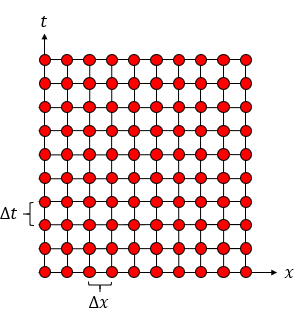
\includegraphics[scale = 0.9]{Discretize.png}
    \caption{Grid where space and time dimensions are discretized by 10 steps.}
\end{figure}

Following step of discretization process is applying the values given by inital and boundary conditions to the set of points on the grid.

\begin{figure}[!htb]
\centering
  \begin{minipage}[b]{0.45\textwidth}
   \centering
     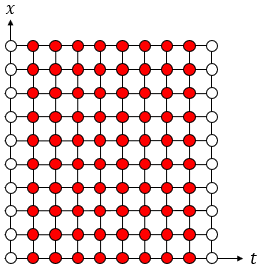
\includegraphics[width=\textwidth]{Boundary.png}
    \caption{Boundary conditions.}
  \end{minipage}
  \begin{minipage}[b]{0.45\textwidth}
   \centering    
    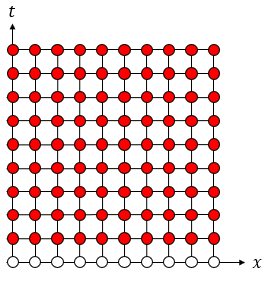
\includegraphics[width=\textwidth]{Initial.png}
    \caption{Initial condition.}
  \end{minipage}
\end{figure}

We need finite difference approximations for the partial derivatives to replace the PDE using the set of points on our grid. Notationally, we will define $u^n_i$ to be a function defined at the point $(i \Delta x, n \Delta t) $.

\begin{itemize}
        \item Forward difference: $ \frac{\partial u}{\partial t} = \frac{u^{n+1}_i - u^n_i}{\Delta t} + \mathcal{O}( \Delta t) $
        \item Central difference: $ \frac{\partial u}{\partial x} = \frac{u^n_{i+1} - u^n_{i-1}}{\Delta t}   + \mathcal{O}( \Delta x) $
        \item Backwards difference: $ \frac{\partial u}{\partial x} = \frac{u^{n}_i - u^n_{i - 1}}{\Delta t}  + \mathcal{O}( \Delta x) $
        \item Second order central difference: $ \frac{\partial^2 u}{\partial x^2} = \frac{u^n_{i+1}- 2u^n_i + u^n_{i-1}}{(\Delta x)^2}  + \mathcal{O}( \Delta x^2) $
\end{itemize}

As we have a grid of points and approximation of the derivatives, it is possible to obtain a unique solution using numerical methods. The implementation of finite difference method class used in this work can be seen under Appendix \ref{FDMClass}.

\subsection{Explicit Method}
Explicit method generalises the parabolic partial differential equation by applying the forward difference to the time derivative and the centred second difference (FTCS scheme).
\begin{equation} \label{gen}
 u_t = a(x, t)  u_{xx} + b(x, t) u_x + c(x, t) u
\end{equation}

We will be applying the finite differences to the equation  \ref{gen}  for the purposes of simplicity since heat equation and Black-Scholes equation can be generalized in the form for certain choices of coefficients. Applying the forward time and centred space differences where $ r = \frac{\Delta t}{\Delta x^2} $.

\begin{eqnarray*}
\frac{u^{n+1}_i - u^n_i}{\Delta t} &=& a(x, t)  \frac{u^n_{i+1}- 2u^n_i + u^n_{i-1}}{(\Delta x)^2}  + b(x, t)  \frac{u^{n}_{i+1} - u^{n}_{i-1}}{\Delta x} + c(x, t) u^n_i \\
u^{n+1}_i &=& u^n_{i + 1} (\frac{-r b(x, t)}{\Delta x} - r a(x, t))\\
&+& u^n_{i}(1 + 2 r a(x, t) - c(x, t) \Delta t) \\
&+& u^n_{i - 1} (-r a(x, t) + \frac{r b(x, t)}{\Delta x})
\end{eqnarray*}


We will replace the coefficients of $ u^n_{i + 1},  u^n_i,  u^n_{i - 1}$  terms with $\gamma,  \alpha, \beta$ respectively. The formula reduces to

\begin{equation}
u_j^{n+1} = \gamma u_{j+1}^{n} + \beta u_{j}^{n} + \alpha u_{j-1}^{n} .
\end{equation}

The formula expresses one unknown nodal value directly in terms of known nodal values  \cite{evans}. It can be expanded as
\begin{multline}
u_1^{n+1} = \gamma u_{2}^{n} + \beta u_{1}^{n} + \alpha u_{0}^{n} \\
u_2^{n+1} = \gamma u_{3}^{n} + \beta u_{2}^{n} + \alpha u_{1}^{n} \\
.\\
\hspace{75pt} .\\
\hspace{150pt} .\\
u_{j-1}^{n+1} = \gamma u_{j}^{n} + \beta u_{j-1}^{n} + \alpha u_{j-2}^{n} 
\end{multline}

\begin{figure}[!htb]
\centering
  \begin{minipage}[b]{0.45\textwidth}
  \centering
    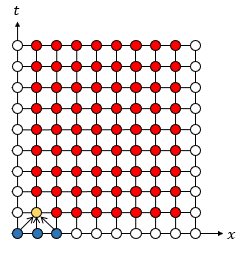
\includegraphics[width=\textwidth]{ExplicitHeat.png}
    \caption{Computational stencil \\of heat equation.}
  \end{minipage}
  \begin{minipage}[b]{0.45\textwidth}
  \centering
    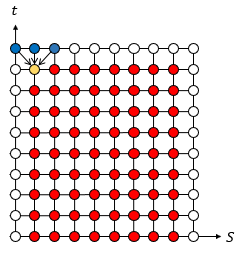
\includegraphics[width=\textwidth]{ExplicitBS.png}
    \caption{Computational stencil \\of Black-Scholes equation.}
  \end{minipage}
\end{figure}

Using the boundary conditions and  initial condition, the expanded formula can be condensed in the following matrix form. 
$$
\begin{bmatrix} 
u_{1}^{n + 1} \\ 
u_{2}^{n + 1} \\ 
u_{3}^{n + 1} \\ 
.\\ 
.\\ 
.\\ 
u_{j - 1}^{n + 1}\\ 
\end{bmatrix} = \begin{bmatrix}
\alpha u_{0}^{n} \\ 
0 \\ 
0 \\ 
.\\ 
.\\ 
.\\ 
\gamma u_{j}^{n} \\ 
\end{bmatrix}  + \begin{bmatrix}  
\beta & \gamma & 0 & . & . & 0 \\ 
\alpha & \beta & \gamma & 0 & ... & . \\ 
0 & \alpha & \beta & \gamma & 0 & . \\ 
. & . & .  & . & . & . \\ 
. & . & .  & . & . & . \\ 
. & . & .  & . & . & \gamma \\ 
0 & 0 & 0 & 0 & \alpha & \beta \\ 
\end{bmatrix} \begin{bmatrix}  
u_{1}^{n} \\ 
u_{2}^{n} \\ 
u_{3}^{n} \\ 
.\\ 
.\\ 
.\\ 
u_{j - 1}^{n} \\ 
\end{bmatrix} 
$$

Deriving the coefficients   $\gamma,  \alpha, \beta$ in the case of heat equation yields
\begin{equation}
\alpha =  r \hspace{15pt} \beta = 1 - 2r \hspace{15pt} \gamma = r
\end{equation}

In the case of Black-Scholes formula, since the share price $S_j$ increases linearly with $\Delta x$ we can replace it as $S_j = j \Delta x$. 
\begin{equation}
\alpha =  \frac{\sigma^2 j^2 \Delta t}{2} - \frac{r j \Delta t}{2} \hspace{15pt} 
\beta = 1 - \sigma^2 j^2 \Delta t - r \Delta t \hspace{15pt} 
\gamma = \frac{\sigma^2 j^2 \Delta t}{2} + \frac{r j \Delta t}{2}
\end{equation}

Lastly, solving heat equation and Black-Scholes differs in time stepping. Black-Scholes formula is solved backwards in time. On the other hand, heat equation is solved forwards in time. 



\begin{figure}[!htb]
  \begin{minipage}[b]{0.5\textwidth}
    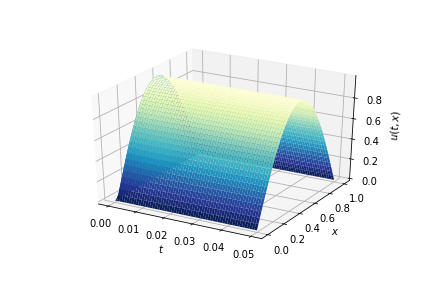
\includegraphics[width=\textwidth]{HeatExplicitGrid.png}
    \caption{Output grid of heat equation using explicit scheme.}
  \end{minipage}
  \begin{minipage}[b]{0.5\textwidth}
    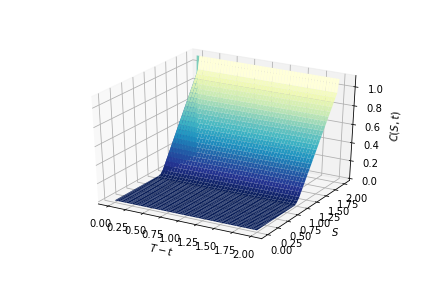
\includegraphics[width=\textwidth]{BSExplicitGrid.png}
    \caption{Output grid of Black-Scholes equation using explicit scheme.}
  \end{minipage}
\end{figure}

\subsection{Crank - Nicolson Method}
The explicit method is computationally cheap. However, this brings a serious drawback, for explicit method to attain reasonable accuracy the step size must be kept small \cite{gdsmith}. Thankfully, the Crank-Nicolson finite difference scheme was introduced by John Crank and Phyllis Nicolson \cite{cn}. In the financial engineering field Crank-Nicolson method is one of the most popular finite difference schemes for calculating numerical solution of the Black-Scholes equation and its variations \cite{tavella}. If we apply backwards time difference instead of forward time difference that Explicit method used and a central space approximation in space again, we get the BTCS scheme. Applying the BTCS to the base equation \ref{gen} yields

\begin{equation}
\frac{u^{n+1}_i - u^n_i}{\Delta t}  = a(x, t)  \frac{u^{n+1}_{i+1}- 2u^{n+1}_i + u^{n+1}_{i-1}}{(\Delta x)^2}  + b(x, t)  \frac{u^{n+1}_i - u^{n+1}_i}{\Delta t}  + c(x, t)  u^{n+1}_i
\end{equation}

Crank - Nicolson method takes a weighted average of the FTCS and BTCS schemes. Therefore, the approximations become
\begin{eqnarray}
u(x, t) &\approx& \frac{1}{2} ( u^{n+1}_i +  u^n_i)\\
\frac{\partial u}{\partial t} &\approx & \frac{u^{n+1}_i - u^n_i}{\Delta t}\\
\frac{\partial u}{\partial x} &\approx & \frac{u^n_{i+1} - u^n_{i-1} + u^{n+1}_{i+1} - u^{n+1}_{i-1}}{4\Delta x} \\ 
\frac{\partial^2 u}{\partial x^2} &\approx & \frac{u^n_{i+1}- 2u^n_i + u^n_{i-1} + u^{n+1}_{i+1}- 2u^{n+1}_i + u^{n+1}_{i-1}}{2(\Delta x)^2}
\end{eqnarray}

Applying the new finite differences to the base partial differential equation equation \ref{gen} yields
\begin{equation}
(-A -B) u^{n+1}_{i+1} + (1 + 2A - C) u^{n+1}_i + (-A + B) u^{n+1}_{i-1} = (A + B) u^{n}_{i+1} + (1 - 2A + C) u^{n}_i + (A - B) u^{n}_{i-1}
\end{equation}

where $ A = a(x, t) \frac{\Delta t}{\Delta x^2}, \hspace{10pt}  B = b(x, t) \frac{\Delta t}{4\Delta x}, \hspace{10pt} C = c(x, t) \frac{\Delta t}{2}$. Note that in contrast to the FTCS scheme, we now have three unknowns in this equation, the three values of $u$ at the higher time level.  We respectively denote the coefficients in the right hand side as $\gamma, \beta, \alpha$ and coefficients in the left hand side as $\lambda, \theta, \omega$ for simplicity.
\begin{equation}
\lambda u^{n+1}_{i+1} + \theta u^{n+1}_i + \omega u^{n+1}_{i-1} \\
=  \gamma u^{n}_{i+1} + \beta u^{n}_i + \alpha u^{n}_{i-1}
\end{equation}

The left hand side groups the unknowns and the right hand side groups knowns. The system of equations can be  reduced to a matrix system.

$$
\begin{bmatrix}  
\theta & \lambda & 0 & . & . & 0 \\ 
\omega & \theta & \lambda & 0 & ... & . \\ 
0 & \omega & \theta & \lambda & 0 & . \\ 
. & . & .  & . & . & . \\ 
. & . & .  & . & . & . \\ 
. & . & .  & . & . & \lambda \\ 
0 & 0 & 0 & 0 & \omega & \theta \\ 
\end{bmatrix}  \begin{bmatrix} 
u_{1}^{n + 1} \\ 
u_{2}^{n + 1} \\ 
u_{3}^{n + 1} \\ 
.\\ 
.\\ 
.\\ 
u_{j - 1}^{n + 1}\\ 
\end{bmatrix}= \begin{bmatrix}
\alpha u_{0}^{n} \\ 
0 \\ 
0 \\ 
.\\ 
.\\ 
.\\ 
\gamma u_{j}^{n} \\ 
\end{bmatrix}  + \begin{bmatrix}  
\beta & \gamma & 0 & . & . & 0 \\ 
\alpha & \beta & \gamma & 0 & ... & . \\ 
0 & \alpha & \beta & \gamma & 0 & . \\ 
. & . & .  & . & . & . \\ 
. & . & .  & . & . & . \\ 
. & . & .  & . & . & \gamma \\ 
0 & 0 & 0 & 0 & \alpha & \beta \\ 
\end{bmatrix} \begin{bmatrix}  
u_{1}^{n} \\ 
u_{2}^{n} \\ 
u_{3}^{n} \\ 
.\\ 
.\\ 
.\\ 
u_{j - 1}^{n} \\ 
\end{bmatrix}
$$

The problem reduces to a tridiagonal matrix system. This system of equations can be solved by various algorithms such as Gaussian elimination or Thomas algorithm.

\begin{figure}[!htb]
  \begin{minipage}[b]{0.5\textwidth}
    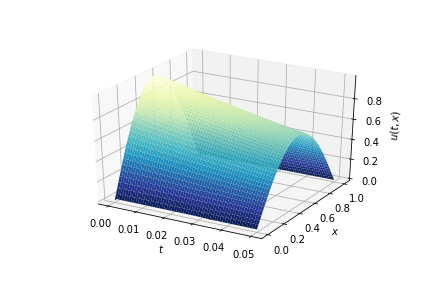
\includegraphics[width=\textwidth]{HeatCNGrid.png}
    \caption{Output grid of heat equation using Crank - Nicolson scheme.}
  \end{minipage}
  \begin{minipage}[b]{0.5\textwidth}
    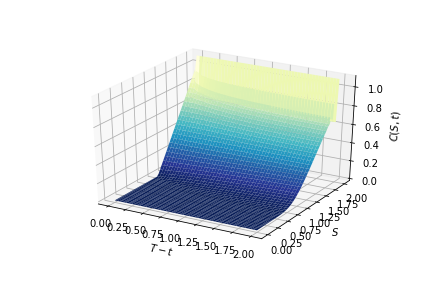
\includegraphics[width=\textwidth]{BSCNGrid.png}
    \caption{Output grid of Black-Scholes equation using Crank - Nicolson scheme.}
  \end{minipage}
\end{figure}

\subsection{Alternating Direction Implicit Method}
Curse of dimensionality effects finite difference schemes as they tend to become more difficult to set up, understand and implement as the dimensionality of the space increases \cite{duffyfinite}. The alternating direction implicit (ADI) method is one of the most common techniques to numerically solve two-dimensional parabolic PDEs. The scheme was first proposed by Peaceman and Rachford in 1955 for oil reservoir modelling \cite{peace}. The method consists of splitting the time dimension and solving the two-dimensional problem as two consecutive one-dimensional problems.  At each time step, the spatial dimensions are solved implicitly in one direction and explicitly in the other dimension. Using the alternating direction implicit scheme provides us with the advantages of implicit method. Computationally requires only solving tridiagonal systems. It is possible to use ADI in more than three dimensions which produce the same number of consecutive one-dimensional problems \cite{DougADI}. To develop a more compact notation, we introduce the finite difference operator notation $\delta^2$.

\begin{equation}
\delta x^2 u^{n}_{i,j}  = \frac{u^{n}_{i+1,j} - 2u^{n}_{i,j} + u^{n}_{i-1,j}}{\Delta x^2}
\end{equation}

Explicit method in two space dimensions can be abbreviated as
\begin{equation}
\frac{u^{n+1}_{i,j} + u^{n}_{i,j}}{\Delta t} = \delta x^2 u^{n}_{i,j} + \delta y^2 u^{n}_{i,j}
\end{equation}
and implicit method in two space dimensions can be written as
\begin{equation}
\frac{u^{n+1}_{i,j} + u^{n}_{i,j}}{\Delta t} = \delta x^2 u^{n+1}_{i,j} + \delta y^2 u^{n+1}_{i,j} .
\end{equation}

Dividing each time step in half we introduce a temporary intermediate unknown $u^{n+1/2}_{i,j}$. Firstly, the two dimensional heat equation is approximating implicitly x and explicitly over y. The total work involved in one time step amounts to solving $ N_{steps} - 1$ tridiagonal systems \cite{morton}. 
\begin{equation}
\frac{u^{n+1/2}_{i,j} + u^{n}_{i,j}}{0.5 \Delta t} = \frac{\delta x^2 u^{n+1/2}_{i,j} }{\Delta x^2} + \frac{\delta y^2 u^{n}_{i,j}}{\Delta y^2}
\end{equation}
Rearranging the set of equations yields a tridiagonal system which is solved for the temporary intermediate unknown $u^{n+1/2}_{i,j}$.
\begin{equation}
- r_x u^{n+1/2}_{i+1,j} + (1 + 2r_x) u^{n+1/2}_{i,j}  - r_x u^{n+1/2}_{i,j}  = r_y u^{n}_{i,j+1} + (1 + 2r_y) u^{n}_{i,j} + r_y u^{n}_{i,j-1}
\end{equation}

\begin{figure}[!htb]
    \centering
        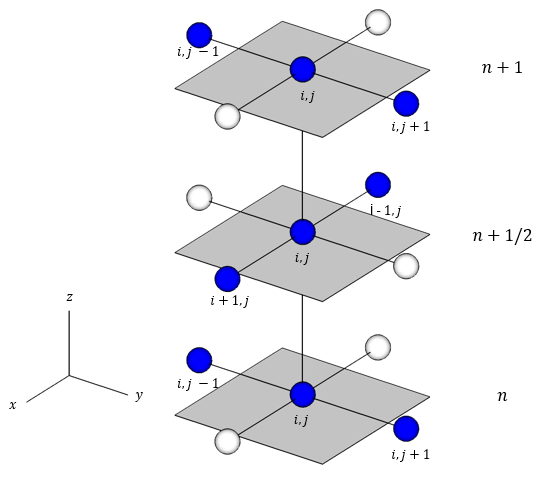
\includegraphics[scale=0.7]{ADI.png}
    \caption{Computational stencil of alternating direction implicit method.}
\end{figure}

Next step of the grid $u^{n+1}_{i,j}$ is calculated by approximating explicitly x and implicitly over y.
\begin{equation}
\frac{u^{n+1}_{i,j} + u^{n+1/2}_{i,j}}{0.5 \Delta t} = \frac{\delta x^2 u^{n+1/2}_{i,j} }{\Delta x^2} + \frac{\delta y^2 u^{n+1}_{i,j}}{\Delta y^2}
\end{equation}

\begin{figure}[!htb]
    \centering
        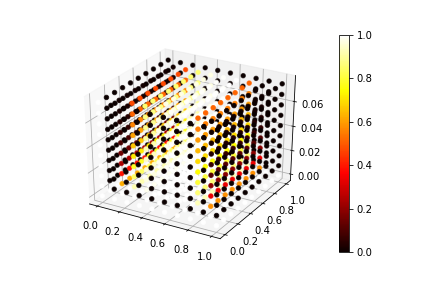
\includegraphics[scale=0.6]{ADIHeat.png}
    \caption{Output grid of two dimensional heat equation using ADI.}
\end{figure}

Rearranging the set of equations yields a tridiagonal system which can be solved using Gaussian elimination, cyclic reduction or Thomas algorithm.
\begin{equation}
-r_y u^{n+1}_{i,j+1} + (1 + 2r_y) u^{n+1}_{i,j} - r_y u^{n+1}_{i,j-1} = r_x * u^{n+1/2}_{i+1,j} + (1 + 2r_x) u^{n+1/2}_{i,j} + r_x u^{n+1/2}_{i,j}
\end{equation}

\chapter{Optimizing Solvers}

Attempting to progress in solving complex problems using numerical methods is impossible without applying optimizations. Nowadays the difficulty is not solving a given problem but rather solving it in a given computing environment while optimally exploiting the resources. Thus, it is necessary to investigate methods that allow for efficient implementations. This section aims to introduce practical optimization techniques that can be easily implemented on a regular trading floor. Main optimization techniques that will be tested are parallelizing tridiagonal solvers, Visual Studio optimization switches, compilers and solution platforms.

\section{Solution Platforms}
The CPU accesses data from RAM using the register that stores memory addresses. 32-bit and 64-bit refer to the amount of data the system can access. so a 32-bit system can address a maximum of 4 GB ($4,294,967,296$ bytes) of RAM where a 64-bit system can access $18,446,744,073,709,551,616$ bytes of memory. Since 32 bit does not have access to more than 4 GB, if the system has more than 4 GB of RAM, it will be inaccessible by the CPU, thus a 64-bit system will be needed. The memory increase of 64 bit systems means it is capable of very fast processing of numerical operations. One disadvantage of the 64 bit systems is more requirement of memory because addresses are 64 bits (8 bytes) wide instead of 32 bits (4 bytes) wide. Due to the increased sizes, 64-bit programs will occupy more memory than a 32-bit version. Visual Studio offers the x86 and x64 solution platforms which corresponds to 32-bit and 64-bit respectively. The solution platforms will be tested against to determine the optimal solution platform.

\section{Compilers}
The software we write is translated into low-level abstractions by a compiler. The quality of translation plays a crucial role in how the software performs. Commonly, compilers are comprised of three stages, front end, optimization and the back end.  The first step is to understand the source code to translate it into intermediate representation using data structures and formal language theory. The intermediate representation generated in the front end is later used by the back end. In the middle, the optimizer is focused on efficiency. It transforms the intermediate representation by deriving knowledge about runtime behaviour and improve the behaviour. Finally, the back end maps the functionality to the instruction set of the processor \cite{compiler}. 

\begin{figure}[!htb]
    \centering
        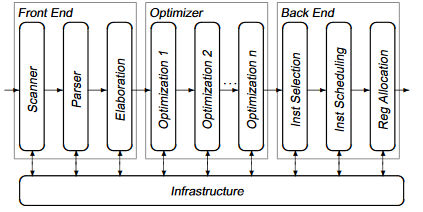
\includegraphics[scale=1]{compiler.png}
    \caption{Basic structure of a compiler.}
\end{figure}

During the back end stage, the compiler approximates the allocation and scheduling. The speed and size of the code is a direct result of the ability to approximate correctly. This produces complex interactions that can lead to problematic results. Therefore, regardless of the implementation of the program, the performance can be different under varying compilers and they are an important factor for time-constrained tasks such as option pricing.  Well designed and implemented compilers savings accumulate over time. It should be able to produce well-optimized code and let us focus on the process of writing programs rather than struggling with the inadequacies of the compiler.  In this project, Visual C++ and Intel C++ compiler will be tested against each other. 

\section{Visual Studio Optimization Switches}
Visual Studio Optimization Switches, also known as /O options controls various optimizations to be chosen according to the needs of the project. There are various switches for different goals such as minimizing the size of the code (/O1) but since the scope of this project is limited with speed optimizations. Speed optimization flags are /O2 and /Ox. /O2 is a combination of /Og, /Oi, /Ot, /Oy, /Ob2, /GF and /Gy flags. /Ox is a subset of /O2 without the  /GF and /Gy flags. These additional options applied by /O2 can cause pointers to strings or to functions to share a target address, which can affect debugging and strict language conformance  \cite{vsopt}. 

\begin{itemize}
\item /Og: Enables local and global optimizations (subexpression elimination), automatic-register allocation, and loop optimization \cite{og}. 
\item /Oi: Generates intrinsic functions for appropriate function calls. Compiler may not replace the function call with an intrinsic if it will result in better performance \cite{oi}.
\item /Ot: Favors optimizations for speed over optimizations for size by instructing the compiler to reduce many C and C++ constructs to functionally similar sequences of machine code. If /Ot is used, /Og must be specified to optimize the code \cite{ot}.
\item /Oy: Suppresses the creation of frame (base) pointers on the call stack for quicker function calls.  Frees one register for general usage \cite{oy}.
\item /Ob2: Controls inline expansion of functions. Under /O2 and /Ox, allows the compiler to expand any function including the ones  that are not explicitly marked for no inlining. Function-calling-overheads are saved thus inline functions run faster than the normal functions with a memory penalty \cite{ob}.
\item /GF:  Enables the compiler to create a single copy of identical strings in the program image and in memory during execution. This is an optimization called string pooling that can create smaller programs. Under this flag, strings are pooled as read-only, trying to modify strings throws an error \cite{gf}.
\item /Gy: Enables function-level linking. Allows the compiler to package individual functions in the form of packaged functions  (COMDATs) or order individual functions in a DLL or .exe file \cite{gy}.
\end{itemize}

/O2 and /Ox flags are tested for maximum speed against the /Od flag which disables all the optimizations.
 
\section{Tridiagonal Solvers}
Tridiagonal solvers are the most demanding part of the solvers. Hence, development and improvement of such solvers is of great interest \cite{terekhov} \cite{chavez} \cite{hofen} \cite{austin} \cite{fpga} concerned with this problem.  Large tridiagonal systems appear in many numerical analysis applications. In our work, they arise in the Crank-Nicolson and Alternating Direction Implicit schemes.  Solving tridiagonal systems is the most computationally intensive part of the schemes. Therefore, choosing efficient tridiagonal solvers is crucial for the speed of the solver. In this experiment, implementations of the Thomas algorithm, Gaussian elimination and cyclic reduction will be tested.

\subsection{Thomas Algorithm}
Thomas Algorithm is the most commonly used method for solving a tridiagonal system of equations. The method is used to solve a tridiagonal matrix system invented by Llewellyn Thomas \cite{thomas}. The algorithm is equivalent to Gaussian elimination without pivoting. The system equations can be written as
$$
\begin{bmatrix}  
b_1 & c_1 & 0 & 0 & ... & 0 \\ 
a_2 & b_2 & c_2 & 0 & ... & 0 \\ 
0 & a_3 & b_3 & c_3 & 0 & 0 \\ 
. & . &  &  &  & . \\ 
. & . &  &  &  & . \\ 
. & . &  &  &  & c_{k-1} \\ 
0 & 0 & 0 & 0 & a_k & b_k \\ 
\end{bmatrix} \begin{bmatrix}  
f_1 \\ 
f_2 \\ 
f_3 \\ 
.\\ 
.\\ 
.\\ 
f_k \\ 
\end{bmatrix} = \begin{bmatrix} 
d_1 \\ 
d_2 \\ 
d_3 \\ 
.\\ 
.\\ 
.\\ 
d_k \\ 
\end{bmatrix}
$$

The method begins by calculating coefficients \(c^{*}_i\) and \(d^{*}_i\) replacing \(a_i\), \(b_i\) and \(c_i\) \cite{duffycpp}.
$$
c^{*}_i = \left\{
     \begin{array}{lr}
       \frac{c_1}{b_1} & ; i = 1\\
       \frac{c_i}{b_i - c^{*}_{i-1} a_i} & ; i = 2,3,...,k-1
     \end{array}
   \right.
$$
$$   
d^{*}_i = \left\{
     \begin{array}{lr}
       \frac{d_1}{b_1} & ; i = 1\\
       \frac{d_i-d^{*}_{i-1} a_i}{b_i - c^{*}_{i-1} a_i} & ; i = 2,3,...,k-1
     \end{array}
   \right.
   $$
The equations can be rewritten as 
$$
\begin{bmatrix}  
1 & c^{*}_1 & 0 & 0 & ... & 0 \\ 
0 & 1 & c^{*}_2 & 0 & ... & 0 \\ 
0 & 0 & 1 & c^{*}_3 & 0 & 0 \\ 
. & . &  &  &  & . \\ 
. & . &  &  &  & . \\ 
. & . &  &  &  & c^{*}_{k-1} \\ 
0 & 0 & 0 & 0 & 0 & 1 \\ 
\end{bmatrix} \begin{bmatrix}  
f_1 \\ 
f_2 \\ 
f_3 \\ 
.\\ 
.\\ 
.\\ 
f_k \\ 
\end{bmatrix} = \begin{bmatrix} 
d^{*}_1 \\ 
d^{*}_2 \\ 
d^{*}_3 \\ 
.\\ 
.\\ 
.\\ 
d^{*}_k \\ 
\end{bmatrix}
$$

The last step is to work in reverse with the following equations.
\[ f_k = d^{*}_k, \qquad f_i = d^{*}_k - c^{*}_i x_{i+1}, \qquad i = k-1, k-2, ... ,2,1 \]

Notice that when solving Thomas Algorithm, it cannot take advantage of parallelism as each step depends on the other element.

\subsection{Intel Math Kernel Library}
Intel Math Kernel Library implements routines for solving systems of linear equations from the standard LAPACK library which is a software package provided by the University of Tennessee. Variety of matrix types are supported by the routines. Specifically, gtsv function is utilized from the package. Using Gaussian elimination with partial pivoting, gstv computes the solution to the system of linear equations with a tridiagonal coefficient matrix \cite{gtsv}.  Gaussian elimination with partial pivoting starts by determining the pivot by finding the largest absolute value at the left column. If necessary, row interchange is performed to ensure that the largest value is at the first-row \cite{gtsvSource}.

$$
\begin{bmatrix}  
b_1 & c_1 & 0 & 0 & ... & 0 \\ 
a_2 & b_2 & c_2 & 0 & ... & 0 \\ 
0 & a_3 & b_3 & c_3 & 0 & 0 \\ 
. & . &  &  &  & . \\ 
. & . &  &  &  & . \\ 
. & . &  &  &  & c_{k-1} \\ 
0 & 0 & 0 & 0 & a_k & b_k \\ 
\end{bmatrix} \begin{bmatrix}  
f_1 \\ 
f_2 \\ 
f_3 \\ 
.\\ 
.\\ 
.\\ 
f_k \\ 
\end{bmatrix} = \begin{bmatrix} 
d_1 \\ 
d_2 \\ 
d_3 \\ 
.\\ 
.\\ 
.\\ 
d_k \\ 
\end{bmatrix}
$$

Assume that the first row is the pivot in the above system of equations. The pivot row is substituted from the second row to eliminate $a_2$. The process of selecting pivot and eliminating an element is repeated until the system of equations is in upper triangular form

$$
\begin{bmatrix}  
b^{*}_1 & c^{*}_1 & 0 & 0 & ... & 0 \\ 
0 & b^{*}_2 & c^{*}_2 & 0  & ...  & 0\\ 
0 & 0 & b^{*}_3 & c^{*}_3 & 0 & 0  \\ 
. & . &  &  &  & . \\ 
. & . &  &  &  & . \\ 
. & . &  &  &  & c^{*}_{k-1} \\ 
0 & 0 & 0 & 0 & 0 & b^{*}_k \\ 
\end{bmatrix} \begin{bmatrix}  
f_1 \\ 
f_2 \\ 
f_3 \\ 
.\\ 
.\\ 
.\\ 
f_k \\ 
\end{bmatrix} = \begin{bmatrix} 
d^{*}_1 \\ 
d^{*}_2 \\ 
d^{*}_3 \\ 
.\\ 
.\\ 
.\\ 
d^{*}_k \\ 
\end{bmatrix}
$$

Once the system is in this form, it is easily solved by back substitution.
 
\subsection{Cyclic Reduction}\label{cyclic}
Cyclic reduction was proposed by R. W. Hockney in the 1960s for solving the resulting linear systems from the  discretization of the Poisson equation \cite{Hockney}. Cyclic reduction consists of two stages, forward reduction and back substitution. Given an $n$ sized system, we will model the matrix as three vectors, lower diagonal \verb!LDiag! of size $n - 1$, diagonal \verb!Diag! of size $n$ and upper diagonal \verb!UDiag! of size $n - 1$. 
$$
\begin{bmatrix}  
b_1 & c_1 & 0 & 0 & ... & 0 \\ 
a_2 & b_2 & c_2 & 0 & ... & 0 \\ 
0 & a_3 & b_3 & c_3 & 0 & 0 \\ 
. & . &  &  &  & . \\ 
. & . &  &  &  & . \\ 
. & . &  &  &  & c_{k-1} \\ 
0 & 0 & 0 & 0 & a_k & b_k \\ 
\end{bmatrix} \begin{bmatrix}  
f_1 \\ 
f_2 \\ 
f_3 \\ 
.\\ 
.\\ 
.\\ 
f_k \\ 
\end{bmatrix} = \begin{bmatrix} 
d_1 \\ 
d_2 \\ 
d_3 \\ 
.\\ 
.\\ 
.\\ 
d_k \\ 
\end{bmatrix}
$$

During the forward reduction stage, at each step $s$ all odd-indexed equations are updated in parallel using the following equations.
\begin{equation}
a_i^{s} f_{i - 2^{s - 1}}^{s} + f_i^{s} + c^{s}  x_{i + 2^{s - 1}} = d_i^s
\end{equation}
are generated where $ i = 2^s, 2^s + 2^s, ... , n$ and $s = 1, 2, ... , \log_2 n$. In the implementation the $i$ and $s$ are respectively denoted by the variables \verb!iReduce! and \verb!Step!.  
\begin{verbatim}
for (Step = 1; Step <= int(log2(size)); Step++)
{
  for (int iReduce = pow(2, Step) - 1; iReduce < Diag.size();
  iReduce += pow(2, Step))
  {
      offset = pow(2, Step - 1);
      iReduceMinus = iReduce - offset;
      iReducePlus = iReduce + offset;
\end{verbatim}

The updated values at each step are 
\begin{eqnarray}
k_1 &=& \frac{ a_{i}^{s - 1}}{b_{i-1}^{s - 1}}, \hspace{30pt} k_2 = \frac{ c_{i}^{s - 1}}{b_{i+1}^{s - 1}} \\
a_i^{s} &=& -a_{i-1}^{s - 1}  k_1, \hspace{30pt} c_i^{s} = -c_{i+1}^{s - 1}  k_2\\
b_i^{s} &=& b_{i}^{s - 1} -c_{i-1}^{s - 1} k_1 - a_{i+1}^{s - 1}  k_2  \\
d_i^{s} &=& d_i^{s - 1} - d_{i- 1}^{s - 1}  k_1 - d_{i + 1}^{s - 1}   k_2
\end{eqnarray}

Thus, the number of unknowns are reduced by half at each step. The same procedure is applied recursively until there remains only one equation with one unknown where $ i = 2^s, 2^s + 2^s, ... , n$ and $s = 1, 2, ... , \log_2 n$. Since we can't determine $i + 1$ when we are updating the last equation, it is treated differently. The loop in the source code continues to update the values with the given equations where $k_1$ and $k_2$ values are stored in the \verb!Temp1! and \verb!Temp2! variables. The \verb!oldResult! vector is used to store the known values and \verb!newResult! is used to store the solution for the unknowns.
\begin{verbatim}
      //Last equation is treated differently
      if (iReduce == Diag.size() - 1)
      {
          Temp1 = LDiag[iReduce] / Diag[iReduceMinus];
          LDiag[iReduce] = -LDiag[iReduceMinus] * Temp1;
          UDiag[iReduce] = 0;
          Diag[iReduce] = Diag[iReduce] - (UDiag[iReduceMinus] * Temp1);
          oldResult[iReduce] = oldResult[iReduce] - oldResult[iReduceMinus]
              * Temp1;
      }
      else
      {
          Temp1 = LDiag[iReduce] / Diag[iReduceMinus];
          Temp2 = UDiag[iReduce] / Diag[iReducePlus];

          LDiag[iReduce] = -LDiag[iReduceMinus] * Temp1;
          UDiag[iReduce] = -UDiag[iReducePlus] * Temp2;
          Diag[iReduce] = Diag[iReduce] - (LDiag[iReducePlus] * Temp2)
               - (UDiag[iReduceMinus] * Temp1);
          oldResult[iReduce] = oldResult[iReduce]
              - (oldResult[iReduceMinus] * Temp1)
              - (oldResult[iReducePlus] * Temp2);
      }
  }
}
\end{verbatim}
\begin{figure}[!htb]
    \centering
        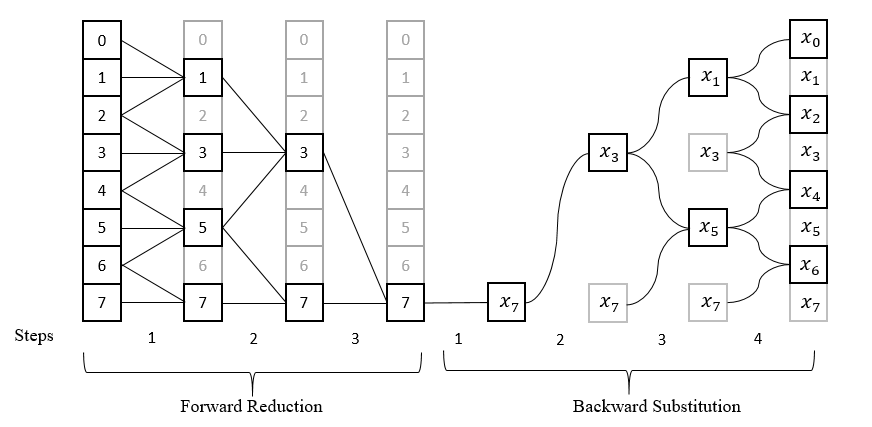
\includegraphics[scale=0.7]{cyclic.png}
    \caption{Cyclic reduction for an eight equation system.}
\end{figure}

After the forward reduction is finished. Backward substitution phase starts where we solve all rest of the unknowns by substituting the already solved value at each time step. As the name implies the steps go backwards as $s = \log_2 n - 1, ... , 0$ and $ i = 2^s, 2^s + 2^{s+1}, ... , n$. Similarly to the forward reduction phase, the $i$ and $s$ variables are stored as \verb!backSub! and \verb!Step!.
\begin{verbatim}
for (int Step = log2(size + 1) - 2; Step >= 0; Step--)
{
    for (int backSub = pow(2, Step + 1) - 1; backSub < size; backSub += pow(2, Step + 1))
    {
        offset = pow(2, Step);
        backSubMinus = backSub - offset;
        backSubPlus = backSub + offset;
\end{verbatim}

The values are determined by the formula at each time step. 
\begin{equation}
f_i = \frac{d_i^{s} - a_i^{s} f_{i - 2^s}  - c_i^{s} f_{i + 2^s}}{b_i^s}
\end{equation}
However, the last and the first equations require a special treatment since they do not have a next or previous element to calculate their solution. The rest of the loop continues as
\begin{verbatim}
      //Special treatment of the first element.
      if (backSubMinus - offset < 0)
      {
          newResult[backSubPlus] = (oldResult[backSubPlus] 
              - (UDiag[backSubPlus] * newResult[backSubPlus + offset])) 
              / Diag[backSubPlus];
      }
      //Special treatment of the last element.
      else if (backSubPlus + offset >= size)
      {
          newResult[backSubMinus] = (oldResult[backSubMinus]
               - (newResult[backSubMinus - offset] * LDiag[backSubMinus]))
               / Diag[backSubMinus];

      }
      else
      {
          newResult[backSubPlus] = (oldResult[backSubPlus] 
              - (newResult[backSubPlus - offset] * LDiag[backSubPlus]) 
              - (UDiag[backSubPlus] * newResult[backSubPlus + offset]))
               / Diag[backSubPlus];
          newResult[backSubMinus] = (oldResult[backSubMinus] 
          - (newResult[backSubMinus - offset] * LDiag[backSubMinus])
          - (UDiag[backSubMinus] * newResult[backSubMinus + offset]))
          / Diag[backSubMinus];
      }
  }
}
\end{verbatim}

If serially computed, Thomas algorithm performs $ 8 n $ operations while cyclic reduction performs $17n$ operations. On the other hand,if parallel computing is used with $n$ cores, cyclic reduction requires $2 \log_2 n - 1$ steps  while the Thomas algorithm requires $2n$ steps \cite{gputri}. The cyclic reduction algorithm was focused towards fine-grained parallelism which could be achieved using CPU parallelism \cite{seltri}.

\section{Open Multi-Processing}
Traditionally, programs are serially computed on a single processor. On the other hand, parallel computation is used to break our code execution in pieces so that it utilizes parallelism. Multithreading uses the CPUs cores to run calculations concurrently in each core. The concurrent programs are called a thread. If the code is executed on parallel processors, one of the biggest problems is the processors generally require results that have been calculated on other processors. The main issue, in this case, is that processors clocks are not synchronized and execute the code at minimally different speeds.

In order to solve this problem, a group of major computer hardware and software vendors and major parallel computing user facilities joined forces to form The Open Multi-Processing Architecture Review Board (The OpenMP ARB)\cite{openmpfaq}. Open Multi-Processing (OpenMP) is an implementation of multithreading for C, C++ and Fortran and it was introduced to public in 1997. OpenMP is aiming to standardize high level parallelism that is performant, productive and portable.

\begin{figure}[!htb]
    \centering
        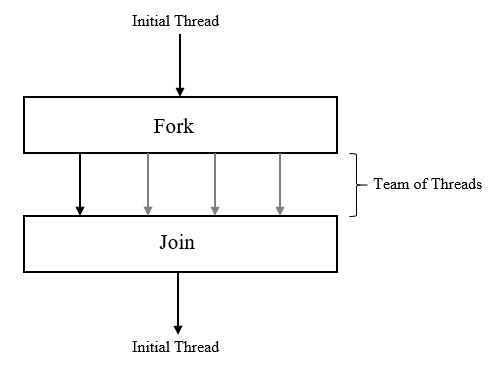
\includegraphics[scale=0.6]{openmp.png}
    \caption{The fork-join programming model.}
\end{figure}

 OpenMP approach to multithreading is the fork-join programming model. Firstly, the program start as a single thread of execution called the initial thread. The fork stage begins when the program encounters an OpenMP parallel construct. Parallel execution takes place and multiple threads are created in the parallel region. The initial thread becomes the master and collaborates with the newly created threads to execute the code dynamically. Finally, at the join stage all threads are synchronized, threads are terminated except the original thread \cite{openmp}.

\begin{figure}[!htb]
    \centering
        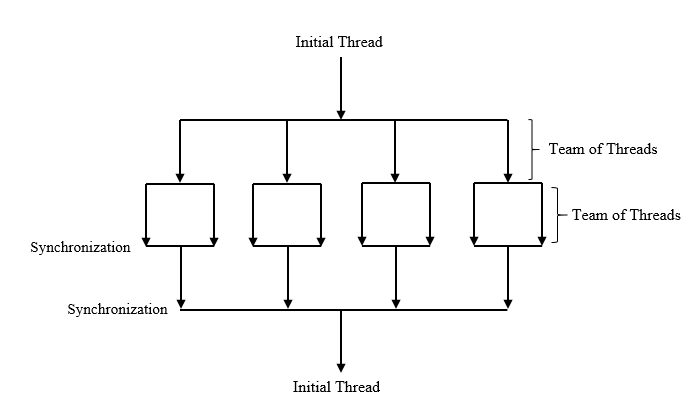
\includegraphics[scale=0.6]{openmpnested.png}
    \caption{4 threads create 2 threads, nested parallelism.}
\end{figure}

Algorithms such as cyclic reduction \ref{cyclic} uses nested loops to calculate the solution. Therefore, nested parallelism is needed to build efficient programs which is achieved by nesting the parallel constructs. Each thread that encounters the next parallel region creates a new parallel region at runtime \cite{openmpnext}.

\begin{figure}[!htb]
    \centering
        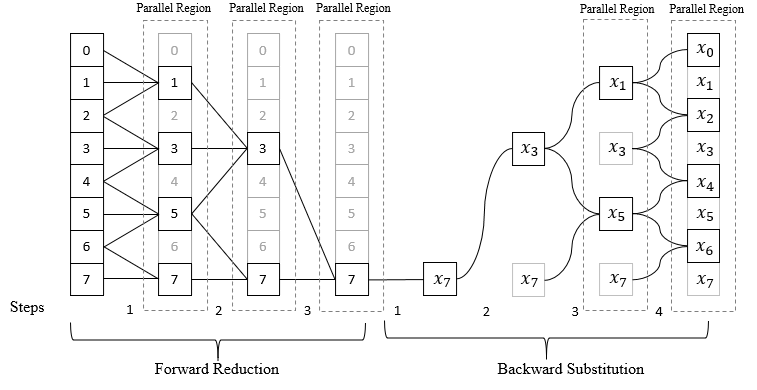
\includegraphics[scale=0.8]{cyclicopenmp.png}
    \caption{Implementation of cyclic reduction using OpenMP.}
\end{figure}

In order to specify and control the parallelization procedure, OpenMP uses compiler directives, runtime functions, and environment variables. OpenMP enables developers to just give a high-level specification of the parallelism by indicating the regions to be executed in parallel using compiler directives, runtime library routines, and environment variables. The details of the parallelism are up to the compiler which makes OpenMP comparatively easy to use. 

\section{Timing the Code}
Timers and clocks might differ on distinct systems. Therefore, measuring execution time intervals accurately is an important task to compare the efficiency and speed of different environments and implementations. 

\subsection{Windows Application Programming Interface}
Windows Application Programming Interface (API) is the lowest level of interaction between applications and the Windows operating system. Thus every program is built upon  the API. Mostly, the interaction is hidden, the runtime and support libraries manage it in the background \cite{windows}. The APIs can be used in the C++ environment. Runtime can be calculated by "QueryPerformanceCounter" or "QueryPerformanceFrequency"  functions. Respectively, the functions retrieve a high resolution time stamp and the frequency of the performance counter. 

\subsection{Chrono Library}
Given the amount of work, using the Windows API for just timing the code is slightly excessive and dependent on the Windows platform. Chrono library was introduced part of the C++11’s standard library. The Chrono library is intended to work with date and time. Chrono library is advantageous since it is platform independent and easy to implement. The \verb!high_resolution_clock! provides the smallest possible tick period and with the \verb!now! method, returns a value corresponding to the call’s point in time. 
\begin{verbatim}
auto Beginning = chrono::high_resolution_clock::now();
    //Portion of code to be timed
auto End = chrono::high_resolution_clock::now();
\end{verbatim}
Once the start and end time of the code is recorded, the duration::count method is used to get the elapsed time. The default setting returns the duration in seconds. Using the \verb!duration\_cast!, the resolution can be converted in hours, minutes, seconds, milliseconds, microseconds and nanoseconds.
\begin{verbatim}
chrono::duration<double> Elapsed = End - Beginning;
// Prints the time in seconds.
cout << "Elapsed time:" << Elapsed.count() << std::endl;
// Prints the time in nanoseconds. 
cout << chrono::duration_cast<chrono::nanoseconds>(Elapsed).count();
\end{verbatim}

An average of 1000 trials is taken to make sure the integrity of timings. Because of the fact that the compiler is clever enough to notice same calculations are repeated, during each execution a random number $ 0 < \epsilon < 10^{-7} $ is added to the step size. 

\chapter{Results and Discussion}
This section documents the performance of attempted optimizations. Experiments are conducted at W307 computer laboratory, Queen Mary University of London. Each computer has Windows 10 Enterprise 64 bit, 16 GB of RAM, Intel Core i7 - 6700 CPU with 4 cores clocked at 3.40 GHz. The source code is written in C++ and compiled with Microsoft Visual Studio Enterprise 2017, Version 15.3.3 in the release mode. External tools utilized in the tests include Intel Compiler, version 18.0.3 and Intel Math Kernel Library. First step was solving the base cases \ref{bsBase}, \ref{HeatBase}, \ref{HeatTwoBase} by hand and Excel. Following the simple implementations, the solvers are ported to C++ to measure and optimize the performance. Different solution platforms, compilers, optimization flags and tridiagonal solvers are tested against each other.
 
\subsection{Base Case}
Previously defined analytical solutions \ref{bsAnal}, \ref{heatAnal}, \ref{heat2Anal} are used to calculate errors for the solutions using different grid sizes. Space and time dimensions are discretized by $64$ for Explicit and Crank - Nicolson schemes. In order to solve two dimensional heat equation using the ADI scheme two space dimensions and the time dimension are discretized by $32$.  All optimizations of Visual Studio  (/Od flag) are disabled for the base case. Following sections summarizes the performance increases by taking average of runtimes. For detailed timings, please refer to the Appendix \ref{timings}.

\begin{figure}[!htb]
    \centering
        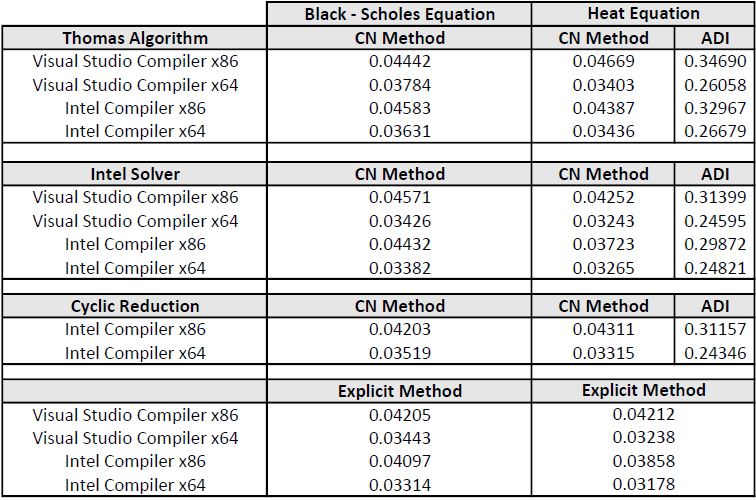
\includegraphics[scale=0.6]{notOptimized.png}
    \caption{Time taken to solve Black - Scholes equation and heat equation using the Explicit, Crank Nicolson and ADI schemes  without any optimization.}
\end{figure}


\subsection{Solution Platforms} 
Switching the solution platform from x86 to x64 resulted in $17 - 22 \%$ decrease in the computing time on average.  The x86 CPU architecture provides $8$ 32-bit general registers and $8$ SSE registers. Using a x64 architecture increases the number of both registers  to $16$. Therefore, calculations are more efficient and fast under 64-bit and we will prefer 64-bit for our best case..

\begin{figure}[!htb]
    \centering
        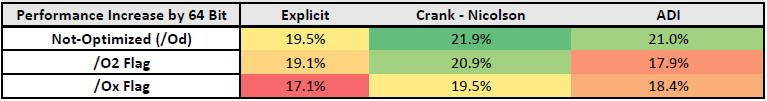
\includegraphics[scale=0.7]{bitPercent.png}
    \caption{Average increase when switched to Intel Compiler under different optimization flags.}
    \label{bitPercent}
\end{figure}



\subsection{Compilers} 
Switching to Intel Compiler provided $0.5 - 4.3 \%$ performance increase on average. 

\begin{figure}[!htb]
    \centering
        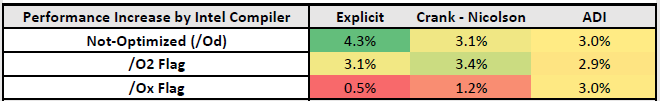
\includegraphics[scale=0.8]{compilerPercent.png}
    \caption{Average increase when switched to Intel compiler.}
\end{figure}

The gtsv function from Intel Math Library was faster under the Intel compiler when compiler optimizations are disabled. However when we enable the /O2 and /Ox optimizations the difference was negligible. The OpenMP support of Visual Studio compiler was not supporting nested for loops. Therefore it is only tested using Intel Compiler. All in all, Intel compiler is faster and provides the support for new technologies such as parallelism. Thus, Intel compiler should be used when dealing with numerical calculations.


\subsection{Visual Studio Optimizations}
The runtime when solving tridiagonal systems greatly benefits from enabling Visual Studio optimizations /Ox and /O2 flags. The Thomas algorithm benefits the most by $10.1 \%$ decrease in runtime on average of  $24$ observations. Similarly, the times for cyclic reduction improved  by $9.5 \%$ on average of $12$ observations. Given the fact that the functions from Intel Math Library are already heavily optimized,  Intel solver improved only $4.6 \%$ on average of $24$ observations. 

\begin{figure}[!htb]
    \centering
    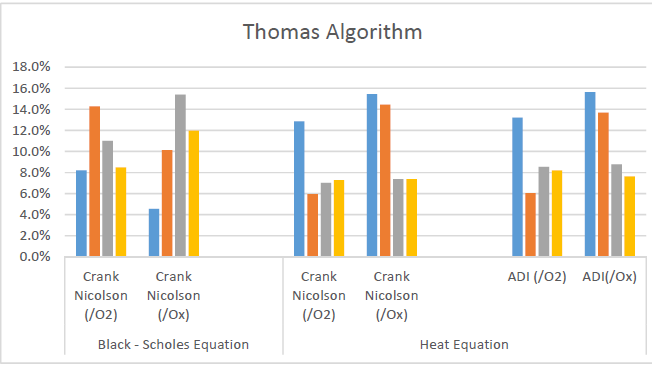
\includegraphics[scale=0.6]{thomasFlagBar.png}
    \caption{The relative performance of optimization switches when using Thomas algorithm.}
\end{figure}

\begin{figure}[!htb]
    \label{intelBar}
    \centering
        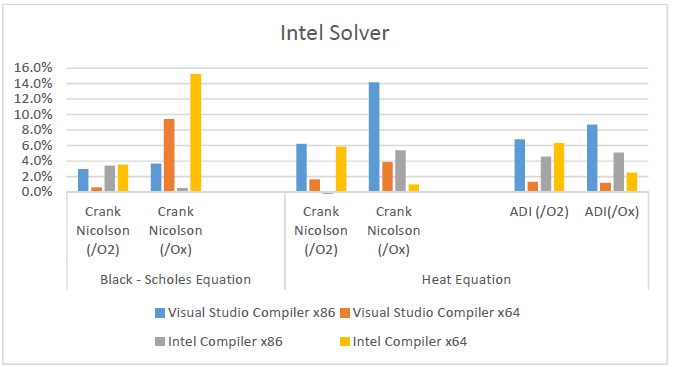
\includegraphics[scale=0.6]{intelFlagBar.png}
    \caption{The relative performance of optimization switches when using Intel solver.}
\end{figure} 

\begin{figure}[!htb]
    \label{cyclicBar}
    \centering
        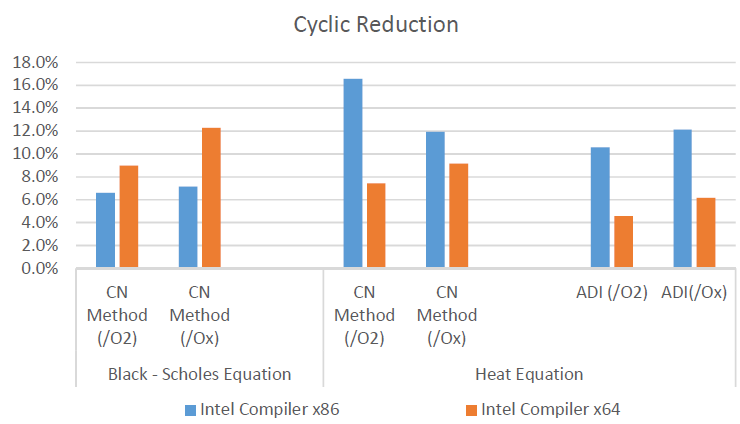
\includegraphics[scale=0.6]{cyclicFlagBar.png}
    \caption{The relative performance of optimization switches when using cyclic reduction.}
\end{figure}

The /Ox switch recorded the fastest times when solving Black - Scholes equation and heat equation regardless of the tridiagonal solvers. Even the explicit method which doesn't require any matrix operations benefited from switching the optimization switches on. The most performance gain recorded by /Ox flag is $13.8 \%$. Overall explicit methods performance improved by $5.4 \%$. Even though the two optimization switches are really close to each other, overall we can conclude that the /Ox flag performs better in the given task  of optimizing schemes. For a detailed view of the performance increases please see the \ref{flagPercent}.

\subsection{Tridiagonal Solvers}
Solving tridiagonal systems is the computationally heaviest component of when calculating solutions with Crank - Nicolson and ADI schemes. Therefore, choosing a fast solver is crucial in our task. Compared to our base case, thomas algorithm, cyclic reduction improved the performance $6.7 \%$ on average. The gtsv function from the Intel Math Library only improved by $0.6 \%$. 

 \begin{figure}[!htb]
    \centering
        \includegraphics[scale=0.7]{solverAveragePercentage.png}
    \caption{Average increase when between solvers.}
\end{figure}
\begin{figure}[!htb]
    \centering
        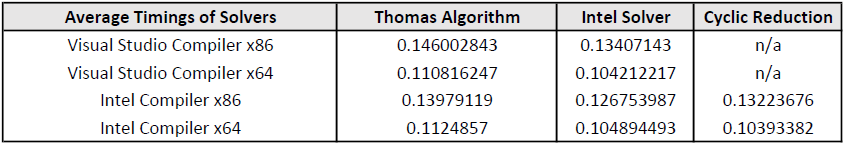
\includegraphics[scale=0.6]{solverAverage.png}
    \caption{Average increase when between solvers timings.}
\end{figure}

Our base case is using x86 platform, Visual Studio compiler, Thomas algorithm and no optimizations. Under these conditions heat equation was solved in $0.046$ seconds and Black - Scholes equation was solved in $0.044$ seconds using the Crank - Nicolson method. The fastest time we achieved is $0.030$ for heat equation and $0.031$ for Black - Scholes equation. Utilizing the Intel compiler, cyclic reduction with OpenMP and /Ox optimization flag resulted in $35.5 \%$ and $30.5 \%$ performance gain for heat equation and Black - Scholes equation. Under the same base case and fastest case conditions the ADI method for two-dimensional heat equation ran in $0.34$ and $0.23$ seconds, resulting in $34.1 \%$ faster solutions.

\subsection{Different Sized Discretizations} 
In the numerical experiments above, the grid size is kept constant. Logically, the performance increase should be greater in case of bigger grids. Therefore, the grid size for Crank - Nicolson method was increase to $128$ by $128$ and $256$ by $256$. Only the base case and fastest case is tested in this section.

 \begin{figure}[!htb]
    \centering
        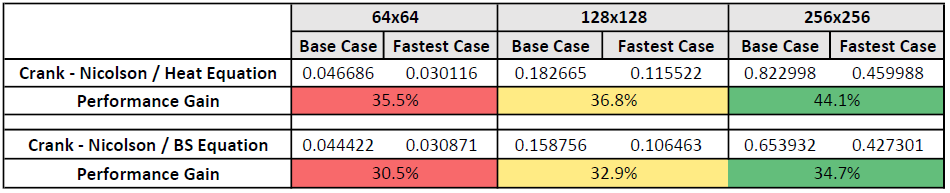
\includegraphics[scale=0.7]{gridTime.png}
    \caption{Average increase when between solvers.}
\end{figure}

As expected, the bigger grid size benefits more from the performance gain. The grid size of ADI method is increased to 64 and 128 from 32 for all dimensions.

 \begin{figure}[!htb]
    \centering
        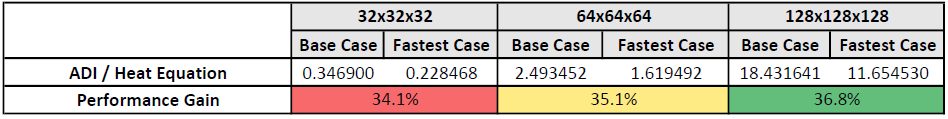
\includegraphics[scale=0.7]{gridTimeADI.png}
    \caption{Average increase when between solvers.}
\end{figure}

Similarly, as the grid size increases the performance gains increase when using ADI method.
\chapter{Conclusion}

Option pricing is a central component for financial corporations, efficient and accurate pricing of them is critical in day to day operations. For  most  partial differential equations, there are no analytical formula giving their price, therefore, numerical methods used to price them. In this thesis, we choose the value options and solve the heat equation to test optimizations for the numerical methods, Crank Nicolson method, explicit method and alternating direction implicit scheme. Numerical analysis and computer simulations are undertaken to put theory and observation together to gain insight into the workings of numerical solutions of partial differential equations. 

The tests in this work suggest that the Intel compiler with 64 bit produces faster code. The Intel compiler provides detailed documentation and support for libraries and tools to develop high-performance programs such as Intel Math Library, Intel Advisor, Intel VTune Performance Analyzer, etc. The timings suggest that the /Ox optimization switch is generally able to provide the best performance. In implementing finite difference methods, we’ve verified that solving tridiagonal systems is the bottleneck. Therefore, we studied the effects of various tridiagonal solvers on the speed of the numerical solution. 
Our results indicate that parallel cyclic reduction is the fastest when using Intel compiler with 64 bit and /Ox switch enabled. 
Against the base case, the best case decrease the timings for Black-Scholes equation and heat equation by $35.5 \%$ and $30.5 \%$. In the two-dimensional heat equation case the fastest solution recorded a  $34.1 \%$ performance gain. Lastly, the effects of optimizations when the grid size changes was studied. 


\subsection{Further Work}
One of the limitations of this project was the type of options. Changing the type of options such as interest rate derivatives and the Black-Scholes model to another pricing framework such as multi asset Black-Scholes or HJM model \cite{kohl} can be implemented. Many optimization techniques have been left for future due to time constraints. The following ideas can provide potential performance improvements
\begin{itemize}
\item Functions and algorithms can be implemented using x86-64 assembly language and the AVX, AVX2, and AVX-512 instruction sets \cite{kusswurm}.
\item General Purpose GPUs can be used with CUDA or Open Computing Language(OpenCL) but can be challenging because of the requirement of delicate memory management.
\item Public cloud-computing services have steadily become cheaper and popular. A cloud function is a serverless execution environment which serves a single function. Building programs on a number of cloud functions is a difficult process. A new study from researchers at Stanford University claims to execute and parallelize existing programs using the cloud functions  \cite{cloudfunc}. Potentially, parallelizing the numerical methods in the cloud can save time and money for financial institutions.
\end{itemize}

\appendix

\chapter{Implementation of the {\tt PDE} class} \label{PDEClass}
Throughout the project, parabolic partial differential equations  are generalised as
\begin{equation} 
 u_t = a(x, t)  u_{xx} + b(x, t) u_x + c(x, t) u
\end{equation}
where $a(x, t)$ denotes diffusion coefficient,  $b(x, t)$ convection coefficient and $c(x, t)$ zero coefficient. Since the coefficients can be functions, each coefficient is implemented as a pure virtual method.

\begin{verbatim}
	virtual double DiffusionCoeff(double t, double x) const = 0;
	virtual double ConvectionCoeff(double t, double x) const = 0;
	virtual double ZeroCoeff(double t, double x) const = 0;
\end{verbatim}

Additionally, initial condition, boundary conditions and analytic solution (if it exists) is implemented in a similar fashion. 

\begin{verbatim}
	virtual double BoundaryLeft(double t, double x) const = 0;
	virtual double BoundaryRight(double t, double x) const = 0;
	virtual double InitCond(double x) const = 0;
	virtual double AnalyticSol(double t, double x) const = 0;
\end{verbatim}


\chapter{Implementation of the {\tt FDM} class} \label{FDMClass}
The FDM class mainly consists of five pure virtual methods to implement finite different schemes. The class also stores step sizes, coefficients for derivative approximations and solutions at the current and previous time step. 

When the class is used, constructor calls \verb!stepSize()! and \verb!initialConditions()!.  
\begin{itemize}
\item \verb!stepSize()! determines step sizes on space and time dimensions. 
\item \verb!initialConditions()!  resizes the solution vectors with respect to the step size and calls the initial condition from the PDE class to fill the vector with initial values.
\item The main difference between schemes is \verb!innerDomain()!  method which updates all solution points. 
\item \verb!boundaryConditions()!  calls the boundary condition from the PDE class and fills the boundary values in the vectors. 
\end{itemize}

The user interacts with the solver using \verb!timeMarch()! method which performs the actual looping of time domain.
A file stream is opened for a csv file. At each time step\verb!innerDomain()! and \verb!boundaryConditions()!  methods are used to calculate the new solution and the result is output to the file. 

\chapter{Detailed Timings} \label{timings}

\begin{figure}[!htb]
    \centering
        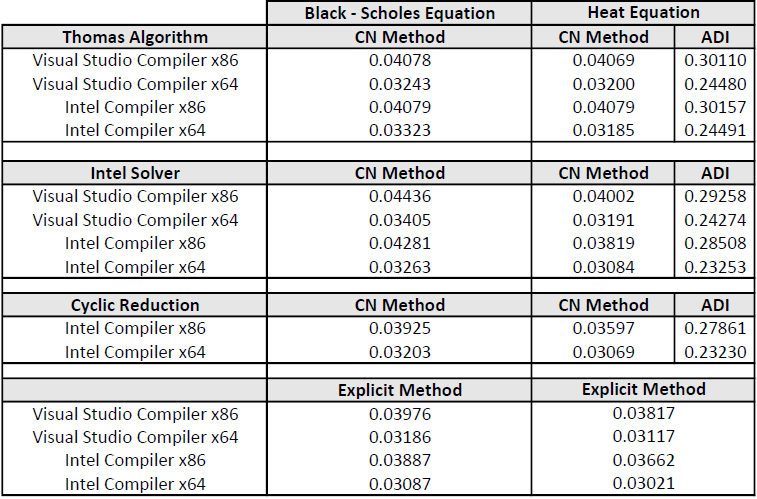
\includegraphics[scale=0.6]{o2Optimized.png}
    \caption{Time taken to solve Black - Scholes equation and heat equation using the Explicit, Crank Nicolson and ADI schemes  optimized with /O2 flag.}
\end{figure}

\begin{figure}[!htb]
    \centering
        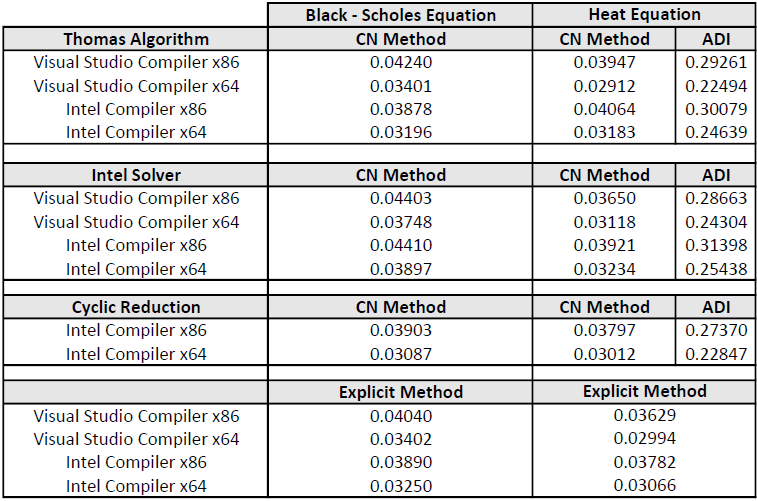
\includegraphics[scale=0.6]{oXOptimized.png}
    \caption{Time taken to solve Black - Scholes equation and heat equation using the Explicit, Crank Nicolson and ADI schemes optimized with /Ox flag.}
\end{figure}

\begin{figure}[!htb]
    \centering
        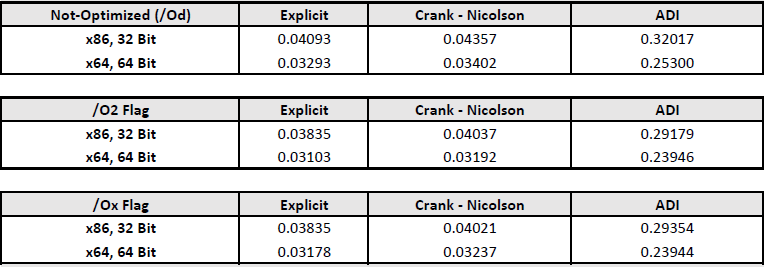
\includegraphics[scale=0.65]{bit.png}
    \caption{Average increase when switched to 64 bit under different optimization flags.}
\end{figure}

\begin{figure}[!htb]
    \centering
        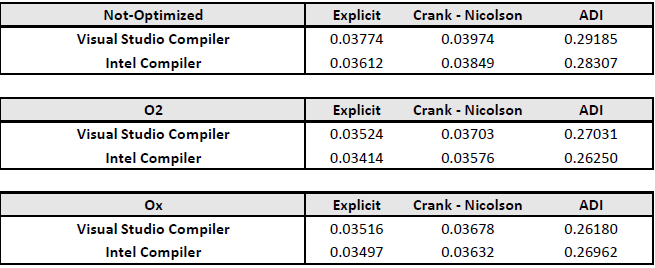
\includegraphics[scale=0.65]{compilerT.png}
    \caption{Average timings comparing Intel Compiler and Visual Studio Compiler.}
\end{figure}

\begin{figure}[!htb]
    \centering
        \includegraphics[scale=0.5]{FlagPercent.png}
    \caption{Percentage decrease in runtime under the /Ox and /O2 flags using the Explicit, Crank Nicolson and ADI schemes .}
    \label{flagPercent}
\end{figure}


\bibliographystyle{plain}
\bibliography{ThesisDraft}

\end{document}
